%\newcommand{\todo}[1]{\todo[color=gray!20,inline]{\textbf{Note}: #1}}
%\makeatletter
%\renewcommand\verbatim@font{\footnotesize\footnotesize\ttfamily}
%\makeatother
%\usepackage[scaled=.8]{nimbusmono}


\documentclass[10pt]{article}
%%%%%%%%%%%%%%%%%%%%%%%%%%%%%%%%%%%%%%%%%%%%%%%%%%%%%%%%%%%%%%%%%%%%%%%%%%%%%%%%%%%%%%%%%%%%%%%%%%%%%%%%%%%%%%%%%%%%%%%%%%%%%%%%%%%%%%%%%%%%%%%%%%%%%%%%%%%%%%%%%%%%%%%%%%%%%%%%%%%%%%%%%%%%%%%%%%%%%%%%%%%%%%%%%%%%%%%%%%%%%%%%%%%%%%%%%%%%%%%%%%%%%%%%%%%%
\usepackage{eurosym}
\usepackage{amsfonts}
\usepackage{amsmath}
\usepackage{booktabs}
\usepackage[a4paper,hmargin={1.4in,1.4in},vmargin={1.4in,1.4in}]{geometry}
\usepackage{mathpazo}
\usepackage[scaled]{helvet}
\usepackage{courier}
\usepackage[T1]{fontenc}
\usepackage{verbatim}
\usepackage{color}
\usepackage{graphicx}
\usepackage{sectsty}
\usepackage{enumitem}
\usepackage{fancyvrb}
\usepackage{newverbs}
\usepackage[bordercolor=white,backgroundcolor=gray!30,linecolor=black]{todonotes}
\usepackage[square,sort,comma,numbers]{natbib}
\usepackage[bookmarks=true,pdfauthor=A.Cesa-Bianchi,colorlinks=true,linkcolor=red,citecolor=note,urlcolor=note]{hyperref}

\setcounter{MaxMatrixCols}{10}
%TCIDATA{OutputFilter=LATEX.DLL}
%TCIDATA{Version=5.50.0.2960}
%TCIDATA{<META NAME="SaveForMode" CONTENT="1">}
%TCIDATA{BibliographyScheme=Manual}
%TCIDATA{LastRevised=Saturday, November 14, 2020 22:51:44}
%TCIDATA{<META NAME="GraphicsSave" CONTENT="32">}
%TCIDATA{Language=American English}

\newlength\myverbindent
\setlength\myverbindent{1cm} \makeatletter
\def\verbatim@processline{  \hspace{\myverbindent}\the\verbatim@line\par}
\makeatother
\definecolor{cmd}{gray}{0.99}
\definecolor{script}{RGB}{255,248,225}
\linespread{1}
\definecolor{subsection}{RGB}{0,0,50}
\definecolor{section}{RGB}{0,0,50}
\definecolor{blue}{RGB}{0,0,100}
\sectionfont{\color{section}}
\subsectionfont{\color{subsection}}
\newenvironment{proof}[1][Proof]{\noindent\textbf{#1.} }{\ \rule{0.5em}{0.5em}}
\renewcommand*\familydefault{\sfdefault}
\graphicspath{{./graphics/}}
\newcommand*\backmatter{\setcounter{section}{0}\renewcommand\theHsection{back.\Roman{section}}}
\definecolor{shadecolor}{rgb}{0.95,0.95,0.95}
\definecolor{title}{RGB}{0,0,90}
\definecolor{note}{RGB}{49,79,179}
\definecolor{light}{RGB}{70,130,180}
\definecolor{red}{RGB}{200,0,0}
\definecolor{gold}{RGB}{218,165,32}
\definecolor{green}{RGB}{0,179,0}
\definecolor{purple}{RGB}{150,40,160}
\definecolor{maroon}{RGB}{128,0,0}
\definecolor{red}{RGB}{140,0,0}
\definecolor{blue}{RGB}{0,0,255}
\definecolor{maroon}{RGB}{128,0,0}
\definecolor{subsection}{RGB}{0,0,90}
\definecolor{section}{RGB}{0,0,90}
\definecolor{matlabgreen}{RGB}{0,153,0}
\definecolor{matlabpurple}{RGB}{127,0,255}
\definecolor{matlabblue}{RGB}{0,42,252}
\sectionfont{\color{section}}
\subsectionfont{\color{subsection}}
\setlength{\parskip}{.25cm}
\setlength{\parindent}{0cm}
\setlist[itemize]{topsep=0cm}
\setlist[itemize]{topsep=0cm}
\renewcommand*\familydefault{\sfdefault}
\renewcommand\labelitemi{-}
\setcounter{secnumdepth}{3}
\graphicspath{{./graphics/}}
% Macros for Scientific Word 2.5 documents saved with the LaTeX filter.
%Copyright (C) 1994-96 TCI Software Research, Inc.
\typeout{TCILATEX Macros for Scientific Word 2.5 <04 SEP 96>.}

\typeout{NOTICE:  This macro file is NOT proprietary and may be 
freely copied and distributed.}


\makeatletter
%%
%% Changes
%% ** to \def\readFRAMEparams
%%    replaces h by H, if the float package is loaded
%%
\@ifundefined{@HHfloat}{\relax}{\typeout{** TCILaTeX detected 'float'-package:}	}	
%%see changes
%
%%%%%%%%%%%%%%%%%%%%%%
% macros for time
\newcount\@hour\newcount\@minute\chardef\@x10\chardef\@xv60
\def\tcitime{
\def\@time{%
  \@minute\time\@hour\@minute\divide\@hour\@xv
  \ifnum\@hour<\@x 0\fi\the\@hour:%
  \multiply\@hour\@xv\advance\@minute-\@hour
  \ifnum\@minute<\@x 0\fi\the\@minute
  }}%

%%%%%%%%%%%%%%%%%%%%%%
% macro for hyperref
\@ifundefined{hyperref}{\def\hyperref#1#2#3#4{#2\ref{#4}#3}}{}

% macro for external program call
\@ifundefined{qExtProgCall}{\def\qExtProgCall#1#2#3#4#5#6{\relax}}{}
%%%%%%%%%%%%%%%%%%%%%%
%
% macros for graphics
%
\def\FILENAME#1{#1}%
%
\def\QCTOpt[#1]#2{%
  \def\QCTOptB{#1}
  \def\QCTOptA{#2}
}
\def\QCTNOpt#1{%
  \def\QCTOptA{#1}
  \let\QCTOptB\empty
}
\def\Qct{%
  \@ifnextchar[{%
    \QCTOpt}{\QCTNOpt}
}
\def\QCBOpt[#1]#2{%
  \def\QCBOptB{#1}
  \def\QCBOptA{#2}
}
\def\QCBNOpt#1{%
  \def\QCBOptA{#1}
  \let\QCBOptB\empty
}
\def\Qcb{%
  \@ifnextchar[{%
    \QCBOpt}{\QCBNOpt}
}
\def\PrepCapArgs{%
  \ifx\QCBOptA\empty
    \ifx\QCTOptA\empty
      {}%
    \else
      \ifx\QCTOptB\empty
        {\QCTOptA}%
      \else
        [\QCTOptB]{\QCTOptA}%
      \fi
    \fi
  \else
    \ifx\QCBOptA\empty
      {}%
    \else
      \ifx\QCBOptB\empty
        {\QCBOptA}%
      \else
        [\QCBOptB]{\QCBOptA}%
      \fi
    \fi
  \fi
}
\newcount\GRAPHICSTYPE
%\GRAPHICSTYPE 0 is for TurboTeX
%\GRAPHICSTYPE 1 is for DVIWindo (PostScript)
%%%(removed)%\GRAPHICSTYPE 2 is for psfig (PostScript)
\GRAPHICSTYPE=\z@
\def\GRAPHICSPS#1{%
 \ifcase\GRAPHICSTYPE%\GRAPHICSTYPE=0
   \special{ps: #1}%
 \or%\GRAPHICSTYPE=1
   \special{language "PS", include "#1"}%
%%%\or%\GRAPHICSTYPE=2
%%%  #1%
 \fi
}%
%
\def\GRAPHICSHP#1{\special{include #1}}%
%
% \graffile{ body }                                  %#1
%          { contentswidth (scalar)  }               %#2
%          { contentsheight (scalar) }               %#3
%          { vertical shift when in-line (scalar) }  %#4
\def\graffile#1#2#3#4{%
%%% \ifnum\GRAPHICSTYPE=\tw@
%%%  %Following if using psfig
%%%  \@ifundefined{psfig}{\input psfig.tex}{}%
%%%  \psfig{file=#1, height=#3, width=#2}%
%%% \else
  %Following for all others
  % JCS - added BOXTHEFRAME, see below
    \leavevmode
    \raise -#4 \BOXTHEFRAME{%
        \hbox to #2{\raise #3\hbox to #2{\null #1\hfil}}}%
}%
%
% A box for drafts
\def\draftbox#1#2#3#4{%
 \leavevmode\raise -#4 \hbox{%
  \frame{\rlap{\protect\tiny #1}\hbox to #2%
   {\vrule height#3 width\z@ depth\z@\hfil}%
  }%
 }%
}%
%
\newcount\draft
\draft=\z@
\let\nographics=\draft
\newif\ifwasdraft
\wasdraftfalse

%  \GRAPHIC{ body }                                  %#1
%          { draft name }                            %#2
%          { contentswidth (scalar)  }               %#3
%          { contentsheight (scalar) }               %#4
%          { vertical shift when in-line (scalar) }  %#5
\def\GRAPHIC#1#2#3#4#5{%
 \ifnum\draft=\@ne\draftbox{#2}{#3}{#4}{#5}%
  \else\graffile{#1}{#3}{#4}{#5}%
  \fi
 }%
%
\def\addtoLaTeXparams#1{%
    \edef\LaTeXparams{\LaTeXparams #1}}%
%
% JCS -  added a switch BoxFrame that can 
% be set by including X in the frame params.
% If set a box is drawn around the frame.

\newif\ifBoxFrame \BoxFramefalse
\newif\ifOverFrame \OverFramefalse
\newif\ifUnderFrame \UnderFramefalse

\def\BOXTHEFRAME#1{%
   \hbox{%
      \ifBoxFrame
         \frame{#1}%
      \else
         {#1}%
      \fi
   }%
}


\def\doFRAMEparams#1{\BoxFramefalse\OverFramefalse\UnderFramefalse\readFRAMEparams#1\end}%
\def\readFRAMEparams#1{%
   \ifx#1\end%
  \let\next=\relax
  \else
  \ifx#1i\dispkind=\z@\fi
  \ifx#1d\dispkind=\@ne\fi
  \ifx#1f\dispkind=\tw@\fi
 	%% BEGIN CHANGES 0.12
	\ifx#1h
    \ifnum\dispkind=\tw@
			\@ifundefined{@HHfloat}{
			  \addtoLaTeXparams{h}
		 	 }{
         \def\LaTeXparams{H}
         \typeout{tcilatex: attribute align pos of FRAME  set to H}
         \typeout{\space \space \space \space all other placement options (tbp) are ignored }
   		 }
	  \else
			\addtoLaTeXparams{h}
    \fi
	\fi
  \if\LaTeXparams H
  	 \ifx#1t\fi	 %% ignore	all other placement
  	 \ifx#1b\fi	 %% options (tbp) 
     \ifx#1p\fi
  \else
      \ifx#1t\addtoLaTeXparams{t}\fi
      \ifx#1b\addtoLaTeXparams{b}\fi
      \ifx#1p\addtoLaTeXparams{p}\fi
  \fi
	%\typeout{LaTeXparms: \LaTeXparams}
%%END CHANGES 0.12

  \ifx#1X\BoxFrametrue\fi
  \ifx#1O\OverFrametrue\fi
  \ifx#1U\UnderFrametrue\fi
  \ifx#1w
    \ifnum\draft=1\wasdrafttrue\else\wasdraftfalse\fi
    \draft=\@ne
  \fi
  \let\next=\readFRAMEparams
  \fi
 \next
 }%
%
%Macro for In-line graphics object
%   \IFRAME{ contentswidth (scalar)  }               %#1
%          { contentsheight (scalar) }               %#2
%          { vertical shift when in-line (scalar) }  %#3
%          { draft name }                            %#4
%          { body }                                  %#5
%          { caption}                                %#6


\def\IFRAME#1#2#3#4#5#6{%
      \bgroup
      \let\QCTOptA\empty
      \let\QCTOptB\empty
      \let\QCBOptA\empty
      \let\QCBOptB\empty
      #6%
      \parindent=0pt%
      \leftskip=0pt
      \rightskip=0pt
      \setbox0 = \hbox{\QCBOptA}%
      \@tempdima = #1\relax
      \ifOverFrame
          % Do this later
          \typeout{This is not implemented yet}%
          \show\HELP
      \else
         \ifdim\wd0>\@tempdima
            \advance\@tempdima by \@tempdima
            \ifdim\wd0 >\@tempdima
               \textwidth=\@tempdima
               \setbox1 =\vbox{%
                  \noindent\hbox to \@tempdima{\hfill\GRAPHIC{#5}{#4}{#1}{#2}{#3}\hfill}\\%
                  \noindent\hbox to \@tempdima{\parbox[b]{\@tempdima}{\QCBOptA}}%
               }%
               \wd1=\@tempdima
            \else
               \textwidth=\wd0
               \setbox1 =\vbox{%
                 \noindent\hbox to \wd0{\hfill\GRAPHIC{#5}{#4}{#1}{#2}{#3}\hfill}\\%
                 \noindent\hbox{\QCBOptA}%
               }%
               \wd1=\wd0
            \fi
         \else
            %\show\BBB
            \ifdim\wd0>0pt
              \hsize=\@tempdima
              \setbox1 =\vbox{%
                \unskip\GRAPHIC{#5}{#4}{#1}{#2}{0pt}%
                \break
                \unskip\hbox to \@tempdima{\hfill \QCBOptA\hfill}%
              }%
              \wd1=\@tempdima
           \else
              \hsize=\@tempdima
              \setbox1 =\vbox{%
                \unskip\GRAPHIC{#5}{#4}{#1}{#2}{0pt}%
              }%
              \wd1=\@tempdima
           \fi
         \fi
         \@tempdimb=\ht1
         \advance\@tempdimb by \dp1
         \advance\@tempdimb by -#2%
         \advance\@tempdimb by #3%
         \leavevmode
         \raise -\@tempdimb \hbox{\box1}%
      \fi
      \egroup%
}%
%
%Macro for Display graphics object
%   \DFRAME{ contentswidth (scalar)  }               %#1
%          { contentsheight (scalar) }               %#2
%          { draft label }                           %#3
%          { name }                                  %#4
%          { caption}                                %#5
\def\DFRAME#1#2#3#4#5{%
 \begin{center}
     \let\QCTOptA\empty
     \let\QCTOptB\empty
     \let\QCBOptA\empty
     \let\QCBOptB\empty
     \ifOverFrame 
        #5\QCTOptA\par
     \fi
     \GRAPHIC{#4}{#3}{#1}{#2}{\z@}
     \ifUnderFrame 
        \nobreak\par #5\QCBOptA
     \fi
 \end{center}%
 }%
%
%Macro for Floating graphic object
%   \FFRAME{ framedata f|i tbph x F|T }              %#1
%          { contentswidth (scalar)  }               %#2
%          { contentsheight (scalar) }               %#3
%          { caption }                               %#4
%          { label }                                 %#5
%          { draft name }                            %#6
%          { body }                                  %#7
\def\FFRAME#1#2#3#4#5#6#7{%
 \begin{figure}[#1]%
  \let\QCTOptA\empty
  \let\QCTOptB\empty
  \let\QCBOptA\empty
  \let\QCBOptB\empty
  \ifOverFrame
    #4
    \ifx\QCTOptA\empty
    \else
      \ifx\QCTOptB\empty
        \caption{\QCTOptA}%
      \else
        \caption[\QCTOptB]{\QCTOptA}%
      \fi
    \fi
    \ifUnderFrame\else
      \label{#5}%
    \fi
  \else
    \UnderFrametrue%
  \fi
  \begin{center}\GRAPHIC{#7}{#6}{#2}{#3}{\z@}\end{center}%
  \ifUnderFrame
    #4
    \ifx\QCBOptA\empty
      \caption{}%
    \else
      \ifx\QCBOptB\empty
        \caption{\QCBOptA}%
      \else
        \caption[\QCBOptB]{\QCBOptA}%
      \fi
    \fi
    \label{#5}%
  \fi
  \end{figure}%
 }%
%
%
%    \FRAME{ framedata f|i tbph x F|T }              %#1
%          { contentswidth (scalar)  }               %#2
%          { contentsheight (scalar) }               %#3
%          { vertical shift when in-line (scalar) }  %#4
%          { caption }                               %#5
%          { label }                                 %#6
%          { name }                                  %#7
%          { body }                                  %#8
%
%    framedata is a string which can contain the following
%    characters: idftbphxFT
%    Their meaning is as follows:
%             i, d or f : in-line, display, or floating
%             t,b,p,h   : LaTeX floating placement options
%             x         : fit contents box to contents
%             F or T    : Figure or Table. 
%                         Later this can expand
%                         to a more general float class.
%
%
\newcount\dispkind%

\def\makeactives{
  \catcode`\"=\active
  \catcode`\;=\active
  \catcode`\:=\active
  \catcode`\'=\active
  \catcode`\~=\active
}
\bgroup
   \makeactives
   \gdef\activesoff{%
      \def"{\string"}
      \def;{\string;}
      \def:{\string:}
      \def'{\string'}
      \def~{\string~}
      %\bbl@deactivate{"}%
      %\bbl@deactivate{;}%
      %\bbl@deactivate{:}%
      %\bbl@deactivate{'}%
    }
\egroup

\def\FRAME#1#2#3#4#5#6#7#8{%
 \bgroup
 \@ifundefined{bbl@deactivate}{}{\activesoff}
 \ifnum\draft=\@ne
   \wasdrafttrue
 \else
   \wasdraftfalse%
 \fi
 \def\LaTeXparams{}%
 \dispkind=\z@
 \def\LaTeXparams{}%
 \doFRAMEparams{#1}%
 \ifnum\dispkind=\z@\IFRAME{#2}{#3}{#4}{#7}{#8}{#5}\else
  \ifnum\dispkind=\@ne\DFRAME{#2}{#3}{#7}{#8}{#5}\else
   \ifnum\dispkind=\tw@
    \edef\@tempa{\noexpand\FFRAME{\LaTeXparams}}%
    \@tempa{#2}{#3}{#5}{#6}{#7}{#8}%
    \fi
   \fi
  \fi
  \ifwasdraft\draft=1\else\draft=0\fi{}%
  \egroup
 }%
%
% This macro added to let SW gobble a parameter that
% should not be passed on and expanded. 

\def\TEXUX#1{"texux"}

%
% Macros for text attributes:
%
\def\BF#1{{\bf {#1}}}%
\def\NEG#1{\leavevmode\hbox{\rlap{\thinspace/}{$#1$}}}%
%
%%%%%%%%%%%%%%%%%%%%%%%%%%%%%%%%%%%%%%%%%%%%%%%%%%%%%%%%%%%%%%%%%%%%%%%%
%
%
% macros for user - defined functions
\def\func#1{\mathop{\rm #1}}%
\def\limfunc#1{\mathop{\rm #1}}%

%
% miscellaneous 
%\long\def\QQQ#1#2{}%
\long\def\QQQ#1#2{%
     \long\expandafter\def\csname#1\endcsname{#2}}%
%\def\QTP#1{}% JCS - this was changed becuase style editor will define QTP
\@ifundefined{QTP}{\def\QTP#1{}}{}
\@ifundefined{QEXCLUDE}{\def\QEXCLUDE#1{}}{}
%\@ifundefined{Qcb}{\def\Qcb#1{#1}}{}
%\@ifundefined{Qct}{\def\Qct#1{#1}}{}
\@ifundefined{Qlb}{\def\Qlb#1{#1}}{}
\@ifundefined{Qlt}{\def\Qlt#1{#1}}{}
\def\QWE{}%
\long\def\QQA#1#2{}%
%\def\QTR#1#2{{\em #2}}% Always \em!!!
%\def\QTR#1#2{\mbox{\begin{#1}#2\end{#1}}}%cb%%%
\def\QTR#1#2{{\csname#1\endcsname #2}}%(gp) Is this the best?
\long\def\TeXButton#1#2{#2}%
\long\def\QSubDoc#1#2{#2}%
\def\EXPAND#1[#2]#3{}%
\def\NOEXPAND#1[#2]#3{}%
\def\PROTECTED{}%
\def\LaTeXparent#1{}%
\def\ChildStyles#1{}%
\def\ChildDefaults#1{}%
\def\QTagDef#1#2#3{}%
%
% Macros for style editor docs
\@ifundefined{StyleEditBeginDoc}{\def\StyleEditBeginDoc{\relax}}{}
%
% Macros for footnotes
\def\QQfnmark#1{\footnotemark}
\def\QQfntext#1#2{\addtocounter{footnote}{#1}\footnotetext{#2}}
%
% Macros for indexing.
\def\MAKEINDEX{\makeatletter\input gnuindex.sty\makeatother\makeindex}%	
\@ifundefined{INDEX}{\def\INDEX#1#2{}{}}{}%
\@ifundefined{SUBINDEX}{\def\SUBINDEX#1#2#3{}{}{}}{}%
\@ifundefined{initial}%  
   {\def\initial#1{\bigbreak{\raggedright\large\bf #1}\kern 2\p@\penalty3000}}%
   {}%
\@ifundefined{entry}{\def\entry#1#2{\item {#1}, #2}}{}%
\@ifundefined{primary}{\def\primary#1{\item {#1}}}{}%
\@ifundefined{secondary}{\def\secondary#1#2{\subitem {#1}, #2}}{}%
%
%
\@ifundefined{ZZZ}{}{\MAKEINDEX\makeatletter}%
%
% Attempts to avoid problems with other styles
\@ifundefined{abstract}{%
 \def\abstract{%
  \if@twocolumn
   \section*{Abstract (Not appropriate in this style!)}%
   \else \small 
   \begin{center}{\bf Abstract\vspace{-.5em}\vspace{\z@}}\end{center}%
   \quotation 
   \fi
  }%
 }{%
 }%
\@ifundefined{endabstract}{\def\endabstract
  {\if@twocolumn\else\endquotation\fi}}{}%
\@ifundefined{maketitle}{\def\maketitle#1{}}{}%
\@ifundefined{affiliation}{\def\affiliation#1{}}{}%
\@ifundefined{proof}{\def\proof{\noindent{\bfseries Proof. }}}{}%
\@ifundefined{endproof}{\def\endproof{\mbox{\ \rule{.1in}{.1in}}}}{}%
\@ifundefined{newfield}{\def\newfield#1#2{}}{}%
\@ifundefined{chapter}{\def\chapter#1{\par(Chapter head:)#1\par }%
 \newcount\c@chapter}{}%
\@ifundefined{part}{\def\part#1{\par(Part head:)#1\par }}{}%
\@ifundefined{section}{\def\section#1{\par(Section head:)#1\par }}{}%
\@ifundefined{subsection}{\def\subsection#1%
 {\par(Subsection head:)#1\par }}{}%
\@ifundefined{subsubsection}{\def\subsubsection#1%
 {\par(Subsubsection head:)#1\par }}{}%
\@ifundefined{paragraph}{\def\paragraph#1%
 {\par(Subsubsubsection head:)#1\par }}{}%
\@ifundefined{subparagraph}{\def\subparagraph#1%
 {\par(Subsubsubsubsection head:)#1\par }}{}%
%%%%%%%%%%%%%%%%%%%%%%%%%%%%%%%%%%%%%%%%%%%%%%%%%%%%%%%%%%%%%%%%%%%%%%%%
% These symbols are not recognized by LaTeX
\@ifundefined{therefore}{\def\therefore{}}{}%
\@ifundefined{backepsilon}{\def\backepsilon{}}{}%
\@ifundefined{yen}{\def\yen{\hbox{\rm\rlap=Y}}}{}%
\@ifundefined{registered}{%
   \def\registered{\relax\ifmmode{}\r@gistered
                    \else$\m@th\r@gistered$\fi}%
 \def\r@gistered{^{\ooalign
  {\hfil\raise.07ex\hbox{$\scriptstyle\rm\text{R}$}\hfil\crcr
  \mathhexbox20D}}}}{}%
\@ifundefined{Eth}{\def\Eth{}}{}%
\@ifundefined{eth}{\def\eth{}}{}%
\@ifundefined{Thorn}{\def\Thorn{}}{}%
\@ifundefined{thorn}{\def\thorn{}}{}%
% A macro to allow any symbol that requires math to appear in text
\def\TEXTsymbol#1{\mbox{$#1$}}%
\@ifundefined{degree}{\def\degree{{}^{\circ}}}{}%
%
% macros for T3TeX files
\newdimen\theight
\def\Column{%
 \vadjust{\setbox\z@=\hbox{\scriptsize\quad\quad tcol}%
  \theight=\ht\z@\advance\theight by \dp\z@\advance\theight by \lineskip
  \kern -\theight \vbox to \theight{%
   \rightline{\rlap{\box\z@}}%
   \vss
   }%
  }%
 }%
%
\def\qed{%
 \ifhmode\unskip\nobreak\fi\ifmmode\ifinner\else\hskip5\p@\fi\fi
 \hbox{\hskip5\p@\vrule width4\p@ height6\p@ depth1.5\p@\hskip\p@}%
 }%
%
\def\cents{\hbox{\rm\rlap/c}}%
\def\miss{\hbox{\vrule height2\p@ width 2\p@ depth\z@}}%
%\def\miss{\hbox{.}}%        %another possibility 
%
\def\vvert{\Vert}%           %always translated to \left| or \right|
%
\def\tcol#1{{\baselineskip=6\p@ \vcenter{#1}} \Column}  %
%
\def\dB{\hbox{{}}}%                 %dummy entry in column 
\def\mB#1{\hbox{$#1$}}%             %column entry
\def\nB#1{\hbox{#1}}%               %column entry (not math)
%
%\newcount\notenumber
%\def\clearnotenumber{\notenumber=0}
%\def\note{\global\advance\notenumber by 1
% \footnote{$^{\the\notenumber}$}}
%\def\note{\global\advance\notenumber by 1
\def\note{$^{\dag}}%
%
%

\def\newfmtname{LaTeX2e}
\def\chkcompat{%
   \if@compatibility
   \else
     \usepackage{latexsym}
   \fi
}

\ifx\fmtname\newfmtname
  \DeclareOldFontCommand{\rm}{\normalfont\rmfamily}{\mathrm}
  \DeclareOldFontCommand{\sf}{\normalfont\sffamily}{\mathsf}
  \DeclareOldFontCommand{\tt}{\normalfont\ttfamily}{\mathtt}
  \DeclareOldFontCommand{\bf}{\normalfont\bfseries}{\mathbf}
  \DeclareOldFontCommand{\it}{\normalfont\itshape}{\mathit}
  \DeclareOldFontCommand{\sl}{\normalfont\slshape}{\@nomath\sl}
  \DeclareOldFontCommand{\sc}{\normalfont\scshape}{\@nomath\sc}
  \chkcompat
\fi

%
% Greek bold macros
% Redefine all of the math symbols 
% which might be bolded	 - there are 
% probably others to add to this list

\def\alpha{{\Greekmath 010B}}%
\def\beta{{\Greekmath 010C}}%
\def\gamma{{\Greekmath 010D}}%
\def\delta{{\Greekmath 010E}}%
\def\epsilon{{\Greekmath 010F}}%
\def\zeta{{\Greekmath 0110}}%
\def\eta{{\Greekmath 0111}}%
\def\theta{{\Greekmath 0112}}%
\def\iota{{\Greekmath 0113}}%
\def\kappa{{\Greekmath 0114}}%
\def\lambda{{\Greekmath 0115}}%
\def\mu{{\Greekmath 0116}}%
\def\nu{{\Greekmath 0117}}%
\def\xi{{\Greekmath 0118}}%
\def\pi{{\Greekmath 0119}}%
\def\rho{{\Greekmath 011A}}%
\def\sigma{{\Greekmath 011B}}%
\def\tau{{\Greekmath 011C}}%
\def\upsilon{{\Greekmath 011D}}%
\def\phi{{\Greekmath 011E}}%
\def\chi{{\Greekmath 011F}}%
\def\psi{{\Greekmath 0120}}%
\def\omega{{\Greekmath 0121}}%
\def\varepsilon{{\Greekmath 0122}}%
\def\vartheta{{\Greekmath 0123}}%
\def\varpi{{\Greekmath 0124}}%
\def\varrho{{\Greekmath 0125}}%
\def\varsigma{{\Greekmath 0126}}%
\def\varphi{{\Greekmath 0127}}%

\def\nabla{{\Greekmath 0272}}
\def\FindBoldGroup{%
   {\setbox0=\hbox{$\mathbf{x\global\edef\theboldgroup{\the\mathgroup}}$}}%
}

\def\Greekmath#1#2#3#4{%
    \if@compatibility
        \ifnum\mathgroup=\symbold
           \mathchoice{\mbox{\boldmath$\displaystyle\mathchar"#1#2#3#4$}}%
                      {\mbox{\boldmath$\textstyle\mathchar"#1#2#3#4$}}%
                      {\mbox{\boldmath$\scriptstyle\mathchar"#1#2#3#4$}}%
                      {\mbox{\boldmath$\scriptscriptstyle\mathchar"#1#2#3#4$}}%
        \else
           \mathchar"#1#2#3#4% 
        \fi 
    \else 
        \FindBoldGroup
        \ifnum\mathgroup=\theboldgroup % For 2e
           \mathchoice{\mbox{\boldmath$\displaystyle\mathchar"#1#2#3#4$}}%
                      {\mbox{\boldmath$\textstyle\mathchar"#1#2#3#4$}}%
                      {\mbox{\boldmath$\scriptstyle\mathchar"#1#2#3#4$}}%
                      {\mbox{\boldmath$\scriptscriptstyle\mathchar"#1#2#3#4$}}%
        \else
           \mathchar"#1#2#3#4% 
        \fi     	    
	  \fi}

\newif\ifGreekBold  \GreekBoldfalse
\let\SAVEPBF=\pbf
\def\pbf{\GreekBoldtrue\SAVEPBF}%
%

\@ifundefined{theorem}{\newtheorem{theorem}{Theorem}}{}
\@ifundefined{lemma}{\newtheorem{lemma}[theorem]{Lemma}}{}
\@ifundefined{corollary}{\newtheorem{corollary}[theorem]{Corollary}}{}
\@ifundefined{conjecture}{\newtheorem{conjecture}[theorem]{Conjecture}}{}
\@ifundefined{proposition}{\newtheorem{proposition}[theorem]{Proposition}}{}
\@ifundefined{axiom}{\newtheorem{axiom}{Axiom}}{}
\@ifundefined{remark}{\newtheorem{remark}{Remark}}{}
\@ifundefined{example}{\newtheorem{example}{Example}}{}
\@ifundefined{exercise}{\newtheorem{exercise}{Exercise}}{}
\@ifundefined{definition}{\newtheorem{definition}{Definition}}{}


\@ifundefined{mathletters}{%
  %\def\theequation{\arabic{equation}}
  \newcounter{equationnumber}  
  \def\mathletters{%
     \addtocounter{equation}{1}
     \edef\@currentlabel{\theequation}%
     \setcounter{equationnumber}{\c@equation}
     \setcounter{equation}{0}%
     \edef\theequation{\@currentlabel\noexpand\alph{equation}}%
  }
  \def\endmathletters{%
     \setcounter{equation}{\value{equationnumber}}%
  }
}{}

%Logos
\@ifundefined{BibTeX}{%
    \def\BibTeX{{\rm B\kern-.05em{\sc i\kern-.025em b}\kern-.08em
                 T\kern-.1667em\lower.7ex\hbox{E}\kern-.125emX}}}{}%
\@ifundefined{AmS}%
    {\def\AmS{{\protect\usefont{OMS}{cmsy}{m}{n}%
                A\kern-.1667em\lower.5ex\hbox{M}\kern-.125emS}}}{}%
\@ifundefined{AmSTeX}{\def\AmSTeX{\protect\AmS-\protect\TeX\@}}{}%
%

%%%%%%%%%%%%%%%%%%%%%%%%%%%%%%%%%%%%%%%%%%%%%%%%%%%%%%%%%%%%%%%%%%%%%%%
% NOTE: The rest of this file is read only if amstex has not been
% loaded.  This section is used to define amstex constructs in the
% event they have not been defined.
%
%
\ifx\ds@amstex\relax
   \message{amstex already loaded}\makeatother\endinput% 2.09 compatability
\else
   \@ifpackageloaded{amstex}%
      {\message{amstex already loaded}\makeatother\endinput}
      {}
   \@ifpackageloaded{amsgen}%
      {\message{amsgen already loaded}\makeatother\endinput}
      {}
\fi
%%%%%%%%%%%%%%%%%%%%%%%%%%%%%%%%%%%%%%%%%%%%%%%%%%%%%%%%%%%%%%%%%%%%%%%%
%%
%
%
%  Macros to define some AMS LaTeX constructs when 
%  AMS LaTeX has not been loaded
% 
% These macros are copied from the AMS-TeX package for doing
% multiple integrals.
%
\def\DN@{\def\next@}%
\def\eat@#1{}%
\let\DOTSI\relax
\def\RIfM@{\relax\ifmmode}%
\def\FN@{\futurelet\next}%
\newcount\intno@
\def\iint{\DOTSI\intno@\tw@\FN@\ints@}%
\def\iiint{\DOTSI\intno@\thr@@\FN@\ints@}%
\def\iiiint{\DOTSI\intno@4 \FN@\ints@}%
\def\idotsint{\DOTSI\intno@\z@\FN@\ints@}%
\def\ints@{\findlimits@\ints@@}%
\newif\iflimtoken@
\newif\iflimits@
\def\findlimits@{\limtoken@true\ifx\next\limits\limits@true
 \else\ifx\next\nolimits\limits@false\else
 \limtoken@false\ifx\ilimits@\nolimits\limits@false\else
 \ifinner\limits@false\else\limits@true\fi\fi\fi\fi}%
\def\multint@{\int\ifnum\intno@=\z@\intdots@                          %1
 \else\intkern@\fi                                                    %2
 \ifnum\intno@>\tw@\int\intkern@\fi                                   %3
 \ifnum\intno@>\thr@@\int\intkern@\fi                                 %4
 \int}%                                                               %5
\def\multintlimits@{\intop\ifnum\intno@=\z@\intdots@\else\intkern@\fi
 \ifnum\intno@>\tw@\intop\intkern@\fi
 \ifnum\intno@>\thr@@\intop\intkern@\fi\intop}%
\def\intic@{%
    \mathchoice{\hskip.5em}{\hskip.4em}{\hskip.4em}{\hskip.4em}}%
\def\negintic@{\mathchoice
 {\hskip-.5em}{\hskip-.4em}{\hskip-.4em}{\hskip-.4em}}%
\def\ints@@{\iflimtoken@                                              %1
 \def\ints@@@{\iflimits@\negintic@
   \mathop{\intic@\multintlimits@}\limits                             %2
  \else\multint@\nolimits\fi                                          %3
  \eat@}%                                                             %4
 \else                                                                %5
 \def\ints@@@{\iflimits@\negintic@
  \mathop{\intic@\multintlimits@}\limits\else
  \multint@\nolimits\fi}\fi\ints@@@}%
\def\intkern@{\mathchoice{\!\!\!}{\!\!}{\!\!}{\!\!}}%
\def\plaincdots@{\mathinner{\cdotp\cdotp\cdotp}}%
\def\intdots@{\mathchoice{\plaincdots@}%
 {{\cdotp}\mkern1.5mu{\cdotp}\mkern1.5mu{\cdotp}}%
 {{\cdotp}\mkern1mu{\cdotp}\mkern1mu{\cdotp}}%
 {{\cdotp}\mkern1mu{\cdotp}\mkern1mu{\cdotp}}}%
%
%
%  These macros are for doing the AMS \text{} construct
%
\def\RIfM@{\relax\protect\ifmmode}
\def\text{\RIfM@\expandafter\text@\else\expandafter\mbox\fi}
\let\nfss@text\text
\def\text@#1{\mathchoice
   {\textdef@\displaystyle\f@size{#1}}%
   {\textdef@\textstyle\tf@size{\firstchoice@false #1}}%
   {\textdef@\textstyle\sf@size{\firstchoice@false #1}}%
   {\textdef@\textstyle \ssf@size{\firstchoice@false #1}}%
   \glb@settings}

\def\textdef@#1#2#3{\hbox{{%
                    \everymath{#1}%
                    \let\f@size#2\selectfont
                    #3}}}
\newif\iffirstchoice@
\firstchoice@true
%
%    Old Scheme for \text
%
%\def\rmfam{\z@}%
%\newif\iffirstchoice@
%\firstchoice@true
%\def\textfonti{\the\textfont\@ne}%
%\def\textfontii{\the\textfont\tw@}%
%\def\text{\RIfM@\expandafter\text@\else\expandafter\text@@\fi}%
%\def\text@@#1{\leavevmode\hbox{#1}}%
%\def\text@#1{\mathchoice
% {\hbox{\everymath{\displaystyle}\def\textfonti{\the\textfont\@ne}%
%  \def\textfontii{\the\textfont\tw@}\textdef@@ T#1}}%
% {\hbox{\firstchoice@false
%  \everymath{\textstyle}\def\textfonti{\the\textfont\@ne}%
%  \def\textfontii{\the\textfont\tw@}\textdef@@ T#1}}%
% {\hbox{\firstchoice@false
%  \everymath{\scriptstyle}\def\textfonti{\the\scriptfont\@ne}%
%  \def\textfontii{\the\scriptfont\tw@}\textdef@@ S\rm#1}}%
% {\hbox{\firstchoice@false
%  \everymath{\scriptscriptstyle}\def\textfonti
%  {\the\scriptscriptfont\@ne}%
%  \def\textfontii{\the\scriptscriptfont\tw@}\textdef@@ s\rm#1}}}%
%\def\textdef@@#1{\textdef@#1\rm\textdef@#1\bf\textdef@#1\sl
%    \textdef@#1\it}%
%\def\DN@{\def\next@}%
%\def\eat@#1{}%
%\def\textdef@#1#2{%
% \DN@{\csname\expandafter\eat@\string#2fam\endcsname}%
% \if S#1\edef#2{\the\scriptfont\next@\relax}%
% \else\if s#1\edef#2{\the\scriptscriptfont\next@\relax}%
% \else\edef#2{\the\textfont\next@\relax}\fi\fi}%
%
%
%These are the AMS constructs for multiline limits.
%
\def\Let@{\relax\iffalse{\fi\let\\=\cr\iffalse}\fi}%
\def\vspace@{\def\vspace##1{\crcr\noalign{\vskip##1\relax}}}%
\def\multilimits@{\bgroup\vspace@\Let@
 \baselineskip\fontdimen10 \scriptfont\tw@
 \advance\baselineskip\fontdimen12 \scriptfont\tw@
 \lineskip\thr@@\fontdimen8 \scriptfont\thr@@
 \lineskiplimit\lineskip
 \vbox\bgroup\ialign\bgroup\hfil$\m@th\scriptstyle{##}$\hfil\crcr}%
\def\Sb{_\multilimits@}%
\def\endSb{\crcr\egroup\egroup\egroup}%
\def\Sp{^\multilimits@}%
\let\endSp\endSb
%
%
%These are AMS constructs for horizontal arrows
%
\newdimen\ex@
\ex@.2326ex
\def\rightarrowfill@#1{$#1\m@th\mathord-\mkern-6mu\cleaders
 \hbox{$#1\mkern-2mu\mathord-\mkern-2mu$}\hfill
 \mkern-6mu\mathord\rightarrow$}%
\def\leftarrowfill@#1{$#1\m@th\mathord\leftarrow\mkern-6mu\cleaders
 \hbox{$#1\mkern-2mu\mathord-\mkern-2mu$}\hfill\mkern-6mu\mathord-$}%
\def\leftrightarrowfill@#1{$#1\m@th\mathord\leftarrow
\mkern-6mu\cleaders
 \hbox{$#1\mkern-2mu\mathord-\mkern-2mu$}\hfill
 \mkern-6mu\mathord\rightarrow$}%
\def\overrightarrow{\mathpalette\overrightarrow@}%
\def\overrightarrow@#1#2{\vbox{\ialign{##\crcr\rightarrowfill@#1\crcr
 \noalign{\kern-\ex@\nointerlineskip}$\m@th\hfil#1#2\hfil$\crcr}}}%
\let\overarrow\overrightarrow
\def\overleftarrow{\mathpalette\overleftarrow@}%
\def\overleftarrow@#1#2{\vbox{\ialign{##\crcr\leftarrowfill@#1\crcr
 \noalign{\kern-\ex@\nointerlineskip}$\m@th\hfil#1#2\hfil$\crcr}}}%
\def\overleftrightarrow{\mathpalette\overleftrightarrow@}%
\def\overleftrightarrow@#1#2{\vbox{\ialign{##\crcr
   \leftrightarrowfill@#1\crcr
 \noalign{\kern-\ex@\nointerlineskip}$\m@th\hfil#1#2\hfil$\crcr}}}%
\def\underrightarrow{\mathpalette\underrightarrow@}%
\def\underrightarrow@#1#2{\vtop{\ialign{##\crcr$\m@th\hfil#1#2\hfil
  $\crcr\noalign{\nointerlineskip}\rightarrowfill@#1\crcr}}}%
\let\underarrow\underrightarrow
\def\underleftarrow{\mathpalette\underleftarrow@}%
\def\underleftarrow@#1#2{\vtop{\ialign{##\crcr$\m@th\hfil#1#2\hfil
  $\crcr\noalign{\nointerlineskip}\leftarrowfill@#1\crcr}}}%
\def\underleftrightarrow{\mathpalette\underleftrightarrow@}%
\def\underleftrightarrow@#1#2{\vtop{\ialign{##\crcr$\m@th
  \hfil#1#2\hfil$\crcr
 \noalign{\nointerlineskip}\leftrightarrowfill@#1\crcr}}}%
%%%%%%%%%%%%%%%%%%%%%

% 94.0815 by Jon:

\def\qopnamewl@#1{\mathop{\operator@font#1}\nlimits@}
\let\nlimits@\displaylimits
\def\setboxz@h{\setbox\z@\hbox}


\def\varlim@#1#2{\mathop{\vtop{\ialign{##\crcr
 \hfil$#1\m@th\operator@font lim$\hfil\crcr
 \noalign{\nointerlineskip}#2#1\crcr
 \noalign{\nointerlineskip\kern-\ex@}\crcr}}}}

 \def\rightarrowfill@#1{\m@th\setboxz@h{$#1-$}\ht\z@\z@
  $#1\copy\z@\mkern-6mu\cleaders
  \hbox{$#1\mkern-2mu\box\z@\mkern-2mu$}\hfill
  \mkern-6mu\mathord\rightarrow$}
\def\leftarrowfill@#1{\m@th\setboxz@h{$#1-$}\ht\z@\z@
  $#1\mathord\leftarrow\mkern-6mu\cleaders
  \hbox{$#1\mkern-2mu\copy\z@\mkern-2mu$}\hfill
  \mkern-6mu\box\z@$}


\def\projlim{\qopnamewl@{proj\,lim}}
\def\injlim{\qopnamewl@{inj\,lim}}
\def\varinjlim{\mathpalette\varlim@\rightarrowfill@}
\def\varprojlim{\mathpalette\varlim@\leftarrowfill@}
\def\varliminf{\mathpalette\varliminf@{}}
\def\varliminf@#1{\mathop{\underline{\vrule\@depth.2\ex@\@width\z@
   \hbox{$#1\m@th\operator@font lim$}}}}
\def\varlimsup{\mathpalette\varlimsup@{}}
\def\varlimsup@#1{\mathop{\overline
  {\hbox{$#1\m@th\operator@font lim$}}}}

%
%%%%%%%%%%%%%%%%%%%%%%%%%%%%%%%%%%%%%%%%%%%%%%%%%%%%%%%%%%%%%%%%%%%%%
%
\def\tfrac#1#2{{\textstyle {#1 \over #2}}}%
\def\dfrac#1#2{{\displaystyle {#1 \over #2}}}%
\def\binom#1#2{{#1 \choose #2}}%
\def\tbinom#1#2{{\textstyle {#1 \choose #2}}}%
\def\dbinom#1#2{{\displaystyle {#1 \choose #2}}}%
\def\QATOP#1#2{{#1 \atop #2}}%
\def\QTATOP#1#2{{\textstyle {#1 \atop #2}}}%
\def\QDATOP#1#2{{\displaystyle {#1 \atop #2}}}%
\def\QABOVE#1#2#3{{#2 \above#1 #3}}%
\def\QTABOVE#1#2#3{{\textstyle {#2 \above#1 #3}}}%
\def\QDABOVE#1#2#3{{\displaystyle {#2 \above#1 #3}}}%
\def\QOVERD#1#2#3#4{{#3 \overwithdelims#1#2 #4}}%
\def\QTOVERD#1#2#3#4{{\textstyle {#3 \overwithdelims#1#2 #4}}}%
\def\QDOVERD#1#2#3#4{{\displaystyle {#3 \overwithdelims#1#2 #4}}}%
\def\QATOPD#1#2#3#4{{#3 \atopwithdelims#1#2 #4}}%
\def\QTATOPD#1#2#3#4{{\textstyle {#3 \atopwithdelims#1#2 #4}}}%
\def\QDATOPD#1#2#3#4{{\displaystyle {#3 \atopwithdelims#1#2 #4}}}%
\def\QABOVED#1#2#3#4#5{{#4 \abovewithdelims#1#2#3 #5}}%
\def\QTABOVED#1#2#3#4#5{{\textstyle 
   {#4 \abovewithdelims#1#2#3 #5}}}%
\def\QDABOVED#1#2#3#4#5{{\displaystyle 
   {#4 \abovewithdelims#1#2#3 #5}}}%
%
% Macros for text size operators:

%JCS - added braces and \mathop around \displaystyle\int, etc.
%
\def\tint{\mathop{\textstyle \int}}%
\def\tiint{\mathop{\textstyle \iint }}%
\def\tiiint{\mathop{\textstyle \iiint }}%
\def\tiiiint{\mathop{\textstyle \iiiint }}%
\def\tidotsint{\mathop{\textstyle \idotsint }}%
\def\toint{\mathop{\textstyle \oint}}%
\def\tsum{\mathop{\textstyle \sum }}%
\def\tprod{\mathop{\textstyle \prod }}%
\def\tbigcap{\mathop{\textstyle \bigcap }}%
\def\tbigwedge{\mathop{\textstyle \bigwedge }}%
\def\tbigoplus{\mathop{\textstyle \bigoplus }}%
\def\tbigodot{\mathop{\textstyle \bigodot }}%
\def\tbigsqcup{\mathop{\textstyle \bigsqcup }}%
\def\tcoprod{\mathop{\textstyle \coprod }}%
\def\tbigcup{\mathop{\textstyle \bigcup }}%
\def\tbigvee{\mathop{\textstyle \bigvee }}%
\def\tbigotimes{\mathop{\textstyle \bigotimes }}%
\def\tbiguplus{\mathop{\textstyle \biguplus }}%
%
%
%Macros for display size operators:
%

\def\dint{\mathop{\displaystyle \int}}%
\def\diint{\mathop{\displaystyle \iint }}%
\def\diiint{\mathop{\displaystyle \iiint }}%
\def\diiiint{\mathop{\displaystyle \iiiint }}%
\def\didotsint{\mathop{\displaystyle \idotsint }}%
\def\doint{\mathop{\displaystyle \oint}}%
\def\dsum{\mathop{\displaystyle \sum }}%
\def\dprod{\mathop{\displaystyle \prod }}%
\def\dbigcap{\mathop{\displaystyle \bigcap }}%
\def\dbigwedge{\mathop{\displaystyle \bigwedge }}%
\def\dbigoplus{\mathop{\displaystyle \bigoplus }}%
\def\dbigodot{\mathop{\displaystyle \bigodot }}%
\def\dbigsqcup{\mathop{\displaystyle \bigsqcup }}%
\def\dcoprod{\mathop{\displaystyle \coprod }}%
\def\dbigcup{\mathop{\displaystyle \bigcup }}%
\def\dbigvee{\mathop{\displaystyle \bigvee }}%
\def\dbigotimes{\mathop{\displaystyle \bigotimes }}%
\def\dbiguplus{\mathop{\displaystyle \biguplus }}%
%
%Companion to stackrel
\def\stackunder#1#2{\mathrel{\mathop{#2}\limits_{#1}}}%
%
%
% These are AMS environments that will be defined to
% be verbatims if amstex has not actually been 
% loaded
%
%
\begingroup \catcode `|=0 \catcode `[= 1
\catcode`]=2 \catcode `\{=12 \catcode `\}=12
\catcode`\\=12 
|gdef|@alignverbatim#1\end{align}[#1|end[align]]
|gdef|@salignverbatim#1\end{align*}[#1|end[align*]]

|gdef|@alignatverbatim#1\end{alignat}[#1|end[alignat]]
|gdef|@salignatverbatim#1\end{alignat*}[#1|end[alignat*]]

|gdef|@xalignatverbatim#1\end{xalignat}[#1|end[xalignat]]
|gdef|@sxalignatverbatim#1\end{xalignat*}[#1|end[xalignat*]]

|gdef|@gatherverbatim#1\end{gather}[#1|end[gather]]
|gdef|@sgatherverbatim#1\end{gather*}[#1|end[gather*]]

|gdef|@gatherverbatim#1\end{gather}[#1|end[gather]]
|gdef|@sgatherverbatim#1\end{gather*}[#1|end[gather*]]


|gdef|@multilineverbatim#1\end{multiline}[#1|end[multiline]]
|gdef|@smultilineverbatim#1\end{multiline*}[#1|end[multiline*]]

|gdef|@arraxverbatim#1\end{arrax}[#1|end[arrax]]
|gdef|@sarraxverbatim#1\end{arrax*}[#1|end[arrax*]]

|gdef|@tabulaxverbatim#1\end{tabulax}[#1|end[tabulax]]
|gdef|@stabulaxverbatim#1\end{tabulax*}[#1|end[tabulax*]]


|endgroup
  

  
\def\align{\@verbatim \frenchspacing\@vobeyspaces \@alignverbatim
You are using the "align" environment in a style in which it is not defined.}
\let\endalign=\endtrivlist
 
\@namedef{align*}{\@verbatim\@salignverbatim
You are using the "align*" environment in a style in which it is not defined.}
\expandafter\let\csname endalign*\endcsname =\endtrivlist




\def\alignat{\@verbatim \frenchspacing\@vobeyspaces \@alignatverbatim
You are using the "alignat" environment in a style in which it is not defined.}
\let\endalignat=\endtrivlist
 
\@namedef{alignat*}{\@verbatim\@salignatverbatim
You are using the "alignat*" environment in a style in which it is not defined.}
\expandafter\let\csname endalignat*\endcsname =\endtrivlist




\def\xalignat{\@verbatim \frenchspacing\@vobeyspaces \@xalignatverbatim
You are using the "xalignat" environment in a style in which it is not defined.}
\let\endxalignat=\endtrivlist
 
\@namedef{xalignat*}{\@verbatim\@sxalignatverbatim
You are using the "xalignat*" environment in a style in which it is not defined.}
\expandafter\let\csname endxalignat*\endcsname =\endtrivlist




\def\gather{\@verbatim \frenchspacing\@vobeyspaces \@gatherverbatim
You are using the "gather" environment in a style in which it is not defined.}
\let\endgather=\endtrivlist
 
\@namedef{gather*}{\@verbatim\@sgatherverbatim
You are using the "gather*" environment in a style in which it is not defined.}
\expandafter\let\csname endgather*\endcsname =\endtrivlist


\def\multiline{\@verbatim \frenchspacing\@vobeyspaces \@multilineverbatim
You are using the "multiline" environment in a style in which it is not defined.}
\let\endmultiline=\endtrivlist
 
\@namedef{multiline*}{\@verbatim\@smultilineverbatim
You are using the "multiline*" environment in a style in which it is not defined.}
\expandafter\let\csname endmultiline*\endcsname =\endtrivlist


\def\arrax{\@verbatim \frenchspacing\@vobeyspaces \@arraxverbatim
You are using a type of "array" construct that is only allowed in AmS-LaTeX.}
\let\endarrax=\endtrivlist

\def\tabulax{\@verbatim \frenchspacing\@vobeyspaces \@tabulaxverbatim
You are using a type of "tabular" construct that is only allowed in AmS-LaTeX.}
\let\endtabulax=\endtrivlist

 
\@namedef{arrax*}{\@verbatim\@sarraxverbatim
You are using a type of "array*" construct that is only allowed in AmS-LaTeX.}
\expandafter\let\csname endarrax*\endcsname =\endtrivlist

\@namedef{tabulax*}{\@verbatim\@stabulaxverbatim
You are using a type of "tabular*" construct that is only allowed in AmS-LaTeX.}
\expandafter\let\csname endtabulax*\endcsname =\endtrivlist

% macro to simulate ams tag construct


% This macro is a fix to eqnarray
\def\@@eqncr{\let\@tempa\relax
    \ifcase\@eqcnt \def\@tempa{& & &}\or \def\@tempa{& &}%
      \else \def\@tempa{&}\fi
     \@tempa
     \if@eqnsw
        \iftag@
           \@taggnum
        \else
           \@eqnnum\stepcounter{equation}%
        \fi
     \fi
     \global\tag@false
     \global\@eqnswtrue
     \global\@eqcnt\z@\cr}


% This macro is a fix to the equation environment
 \def\endequation{%
     \ifmmode\ifinner % FLEQN hack
      \iftag@
        \addtocounter{equation}{-1} % undo the increment made in the begin part
        $\hfil
           \displaywidth\linewidth\@taggnum\egroup \endtrivlist
        \global\tag@false
        \global\@ignoretrue   
      \else
        $\hfil
           \displaywidth\linewidth\@eqnnum\egroup \endtrivlist
        \global\tag@false
        \global\@ignoretrue 
      \fi
     \else   
      \iftag@
        \addtocounter{equation}{-1} % undo the increment made in the begin part
        \eqno \hbox{\@taggnum}
        \global\tag@false%
        $$\global\@ignoretrue
      \else
        \eqno \hbox{\@eqnnum}% $$ BRACE MATCHING HACK
        $$\global\@ignoretrue
      \fi
     \fi\fi
 } 

 \newif\iftag@ \tag@false
 
 \def\tag{\@ifnextchar*{\@tagstar}{\@tag}}
 \def\@tag#1{%
     \global\tag@true
     \global\def\@taggnum{(#1)}}
 \def\@tagstar*#1{%
     \global\tag@true
     \global\def\@taggnum{#1}%  
}

% Do not add anything to the end of this file.  
% The last section of the file is loaded only if 
% amstex has not been.



\makeatother
\endinput

\begin{document}


\section{Installing the VAR Toolbox}

No installation is required. Simply extract the codes from the\ ZIP\ file
and copy them to a specific folder, e.g. \textquotedblleft \texttt{%
C:/UserFolder/VARToolbox}\textquotedblright . Then, add the folder (with
subfolders)\ to the Matlab path. To avoid clashes with other function it is
recommendable to add and remove the Toolbox with the following commands at
beginning and end of your scripts:

\todo[color=script!80,inline]{\ttfamily
addpath(genpath('C:/AMPER/VARToolbox'))

...

rmpath(genpath('C:/AMPER/VARToolbox'))}

To save Figures in high quality format, Ghostscript is needed\ (freely
available at \ \url{www.ghostscript.com}). The VT 3.0 has been tested with
Matlab R2016B on a Windows 10 machine.

\section{VAR Toolbox:\ High level description}

The VAR Toolbox is a collection of Matlab routines to perform VAR analysis.
Vector autoregressive models (VARs) are one of the most successful,
flexible, and easy to use models for the analysis of multivariate time
series. It is a natural extension of the univariate autoregressive model to
dynamic multivariate time series. In their well-known paper
\textquotedblleft Vector Autoregressions,\textquotedblright\ \cite%
{StockWatson2000} describe VAR models as especially useful (and successful)
tools for i) describing the dynamic behavior of economic and financial time
series and ii) for forecasting.

In addition to data description and forecasting, VAR models are also used
for iii) structural inference and iv) policy analysis. In structural
analysis, we generally need to impose certain assumptions about the causal
structure of the data under investigation. The resulting \textquotedblleft
structural\textquotedblright\ VAR\ model can then be used to analyze the
impact of unexpected shocks to specified variables on all the variables in
the model. This is normally done by means of {i{impulse responses}}, {%
forecast error variance decompositions}, and {historical decompositions}.

The VAR Toolbox allows for identification of structural shocks with zero
short-run restrictions; zero long-run restrictions; sign restrictions; and
with the external instrument approach (proxy SVAR). Impulse Response
Functions (IR), Forecast Error Variance Decomposition (VD), and Historical
Decompositions (HD) are computed according to the chosen identification.
Error bands are obtained with bootstrapping. The VAR Toolbox makes use of
few Matlab routines from the Econometrics Toolbox for Matlab by James P.
LeSage (freely available at \url{www.spatial-econometrics.com}).

It also includes a collection of Matlab routines that allows the user to
save and export high quality images from Matlab (using the Export\_fig
function by Oliver Woodford, freely available at %
\url{https://www.mathworks.com/matlabcentral/fileexchange/23629-export_fig}%
). To enable this option, the Toolbox requires Ghostscript installed on your
computer (freely available at \url{www.ghostscript.com}).

The VAR\ Toolbox is not meant to be efficient, but rather to be transparent
and allow the user to understand the econometrics of VARs step by step. The
codes are grouped in six categories (and respective folders):

\begin{itemize}
\item \textbf{Auxiliary}:\ codes that I borrowed from other public sources.
Each m-file has a reference to the original source.

\item \textbf{ExportFig}: this is a toolbox available at Oliver Woodford
website for exporting high quality figures. [add website]

\item \textbf{Figure}:\ codes for plotting high quality figures,
particularly thought for time series. For example, the functions in this
folder allow to efficiently add dates to the x-axis, to control the size and
font of Figures and the appearance of the legends, to plot charts with
shaded error bands, etc.

\item \textbf{Stats}: codes for the calculation of summary statistics,
moving correlations, pairwise correlations, etc.

\item \textbf{Utils}: codes that allow the smooth functioning if the Toolbox.

\item \textbf{VAR}:\ the codes for VAR estimation, identification,
computation of the impulse response functions, FEVD, HD.
\end{itemize}

The idea of this manual is to explain the functioning of the VT\ by means of
a simple example -- the idea being that is much easier to learn by doing
rather than reading a technical manual and then go to the computer. As a
result, many of the functions included in the VT\ are not covered in this
manual, nor is a full description of the output of each function. Moreover,
I\ will need to stop every now and then to introduce some concepts and/or
notation. Sections that include technical details, derivations, etc will be
labelled with {\color{note} {\small {[Note]}}}, while sections that include
details on the practical example will be labelled with {%
\color{note} {\small
{[Matlab]}}}.

Additional resources are available on my website:

\begin{itemize}
\item \url{https://sites.google.com/site/ambropo/replications} provide some
lecture notes on the basics of VARs that are a good complement to this
manual.

\item \url{https://sites.google.com/site/ambropo/matlab-examples} provides a
few examples on how to estimate VARs with different identification schemes
(in a similar spirit to the example in this manual).

\item \url{https://sites.google.com/site/ambropo/replications} provide the
replication codes for a few well-known VAR\ studies (e.g. \cite%
{StockWatson2000}, \cite{BlanchardQuah1989}, \cite{Uhlig2005}, and \cite%
{GertlerKaradi2015}).
\end{itemize}

I will start by introducing some (very light)\ notation.

\section{VAR basics {\color{note} {\protect\small
{[Notes]}} \label%
{sec:basics}}}

Notation, VAR\ structural and reducd-form representation, impulse responses,
variance decompositions, and historical decompositions

\subsection{Vector Autoregressions}

Given a $k\times 1$ vector of time series ($x_{t}$) a Structural Vector
Autoregression (SVAR) of order $p$ can be written as:%
\begin{equation}
x_{t}=\sum_{j=1}^{p}\Phi _{j}x_{t-j}+B\varepsilon _{t},
\label{eq:struct_var_0}
\end{equation}%
where $B$ is a $k\times k$ matrix, generally referred to as \textbf{%
structrual impact matrix}; and $\varepsilon _{t}$ is a $k\times 1$ vector of
serially uncorrelated innovations, generally referred to as \textbf{%
structural shocks}, which are assumed to be mutually uncorrelated and $i.i.d.
$ with zero mean and unit variance.\footnote{%
Note that the fact that the variance of the structural shocks is equal to
one is just a harmless normalization which does not involve a loss of
generality (as long as the diagonal elements of $B$ remain unrestricted. An
alternative (and equivalently valid) normalization would be to leave
unrestricted the variance of the structural innovations, namely $\varepsilon
_{it}\sim \mathcal{N}(0,\sigma _{i}^{2})$ and assume tha the diagonal
elements of $B$ to $1$.}

You should think of the system of equations defined by the structural VAR\
() as approximating the true structure of the economy (for example, the
structure of a DSGE\ model); and the structural shocks as having a
well-defined economic interpretation (for example, TFP\ shocks or monetary
policy shocks).

To keep the notation as simple as possible, consider a bivariate VAR(1),
i.e. a VAR where the number of variables is $k=2$ and the number of lags is $%
p=1$. Also, to make a concrete example, let the two endogenous variables be
output growth ($y_{t}$) and a short-term safe interest rate ($r_{t}$); and
the two structural shocks be a demand shock $\varepsilon _{t}^{Demand}$) and
a monetary policy shock\ ($\varepsilon _{t}^{Mon.\ Pol}$).\footnote{%
Note that this specification is too parsimoniuos to be realistic. But it is
going to simplify the exposition.} This simple bivariate VAR(1) can be
written as a system of linear equations:%
\begin{equation}
\begin{bmatrix}
y_{t} \\
r_{t}%
\end{bmatrix}%
=%
\begin{bmatrix}
\phi _{11} & \phi _{12} \\
\phi _{21} & \phi _{22}%
\end{bmatrix}%
\begin{bmatrix}
y_{t-1} \\
r_{t-1}%
\end{bmatrix}%
+%
\begin{bmatrix}
b_{11} & b_{12} \\
b_{21} & b_{22}%
\end{bmatrix}%
\begin{bmatrix}
\varepsilon _{t}^{Demand} \\
\varepsilon _{t}^{Mon.\ Pol}%
\end{bmatrix}%
,  \label{eq:struct_var_1}
\end{equation}%
or:%
\begin{equation}
\begin{array}{c}
y_{t}=\phi _{11}y_{t-1}+\phi _{12}r_{t-1}+b_{11}\varepsilon
_{t}^{Demand}+b_{12}\varepsilon _{t}^{Mon.\ Pol}, \\
r_{t}=\phi _{21}y_{t-1}+\phi _{22}r_{t-1}+b_{21}\varepsilon
_{t}^{Demand}+b_{22}\varepsilon _{t}^{Mon.\ Pol},%
\end{array}
\label{eq:struct_var_2}
\end{equation}%
where $\varepsilon _{t}=(\varepsilon _{t}^{Demand\prime },\varepsilon
_{t}^{Mon.\ Pol\prime })^{\prime }$ is a $2\times 1$ vector of
(unobservable)\ uncorrelated, zero mean, white noise processes. That is:%
\begin{equation}
\mathbb{V}(\varepsilon _{t})\equiv \Sigma _{\varepsilon }=\left[
\begin{array}{cc}
1 & 0 \\
0 & 1%
\end{array}%
\right] =I_{2}.  \label{eq:struct_cov_1}
\end{equation}%
The assumption that the elements of $\varepsilon _{t}$ are mutually
uncorrelated is crucial. It implies that we can track the effects of a shock
to, say, $\varepsilon _{t}^{Demand}$ to all variables in the VAR keeping the
other shock to zero (and vice versa). The $B$ matrix is also crucial.\ To
see that, consider a unit surprise in $\varepsilon _{t}^{Mon.\ Pol}$, i.e. a
surprise tightening in monetary policy. What are the consequences for output
grpwth $y_{t}$ and $r_{t}$? The answer to this question is in the second
column of the $B$ matrix: $y_{t}$ will move by $b_{12}$ and $r_{t}$ will
move by $b_{22}$. This is why the $B$ matrix is also known as the structural
impact matrix. The $\Phi $ matrix can then be used to track the dynamic
effects of the shocks in $t+1$, $t+2$, etc.

While all this sounds easy and great, there is a complication. The
structural innovations $\varepsilon _{t}$ are unobservable, which means that
we can't directly estimate (\ref{eq:struct_var_2}). The best we can do is to
`bundle' the $\varepsilon _{t}$ into a single object, the \textbf{%
reduced-form innovations}:%
\begin{equation}
\begin{array}{c}
u_{yt}=b_{11}\varepsilon _{t}^{Demand}+b_{12}\varepsilon _{t}^{Mon.\ Pol},
\\
u_{rt}=b_{21}\varepsilon _{t}^{Demand}+b_{22}\varepsilon _{t}^{Mon.\ Pol}.%
\end{array}
\label{eq:red_resid_1}
\end{equation}%
The reduced-form innovations $u_{t}=\left( u_{yt}^{\prime },u_{rt}^{\prime
}\right) ^{\prime }$ are a linear combination of the structural innovations.
We can then rewrite our VAR\ as:%
\begin{equation}
\begin{array}{c}
y_{t}=\phi _{11}y_{t-1}+\phi _{12}r_{t-1}+u_{yt}, \\
r_{t}=\phi _{21}y_{t-1}+\phi _{22}r_{t-1}+u_{rt},%
\end{array}
\label{eq:red_var_0}
\end{equation}%
The VAR in (\ref{eq:red_var_0}) is typically referred to as the \textbf{%
reduced-form representation} of the structural VAR, which can be written
more compactly in matrix form as:%
\begin{equation}
\left[
\begin{array}{c}
y_{t} \\
r_{t}%
\end{array}%
\right] =%
\begin{bmatrix}
\phi _{11} & \phi _{12} \\
\phi _{21} & \phi _{22}%
\end{bmatrix}%
\left[
\begin{array}{c}
y_{t-1} \\
r_{t-1}%
\end{array}%
\right] +\left[
\begin{array}{c}
u_{yt} \\
u_{rt}%
\end{array}%
\right]   \label{eq:red_var_1}
\end{equation}%
where:%
\begin{equation}
\left[
\begin{array}{c}
u_{yt} \\
u_{rt}%
\end{array}%
\right] =%
\begin{bmatrix}
b_{11} & b_{12} \\
b_{21} & b_{22}%
\end{bmatrix}%
\begin{bmatrix}
\varepsilon _{t}^{Demand} \\
\varepsilon _{t}^{Mon.\ Pol}%
\end{bmatrix}%
,  \label{eq:red_resid_2}
\end{equation}%
or:%
\begin{equation}
x_{t}=\Phi x_{t-1}+u_{t}  \label{eq:red_var_2}
\end{equation}%
where $u_{t}=B\varepsilon _{t}$. Differently from the structural VAR\ (\ref%
{eq:struct_var_2}), the parameters of the reduced form VAR\ ($\Phi $) and
its innovations ($u_{t}$) can be estimated with OLS.

The key difference between the structural and reduced for VARs lies in the
covariance matrix of their innovations. While the covariance matrix of the
structural VAR\ innovations is diagonal ($\Sigma _{\varepsilon }=I_{2}$), in
general the covariance reduced form VAR\ innovations are correlated among
themselves, which implies%
\begin{equation}
\mathbb{V}(u_{t})\equiv \Sigma _{u}=\left[
\begin{array}{cc}
\sigma _{y}^{2} & \sigma _{yr}^{2} \\
\sigma _{yr}^{2} & \sigma _{r}^{2}%
\end{array}%
\right] .  \label{eq:red_cov_1}
\end{equation}%
In other words, $\Sigma _{u}$ is a symmetric non-diagonal matrix, where its
diagonal elements are the variances of the estimated reduced-form error
terms, $\sigma _{y}^{2}$ and $\sigma _{r}^{2}$; and the identical
off-diagonal elements are instead equal to the covariance between the
estimated reduced form residuals, $\sigma _{yr}^{2}$\smallskip .

The covariance between the estimated reduced form residuals plays an
important role VARs because it collects the information on the
contemporaneous interaction of the variables in the structural system, which
(as we have just seen) is summarized by the $B$ matrix. Indeed, using (\ref%
{eq:red_resid_2}) the covariance matrix of the reduced for residuals can be
written as:%
\begin{equation}
\Sigma _{u}=\mathbb{E}\left[ u_{t}u_{t}^{\prime }\right] =B\mathbb{E}\left[
\varepsilon _{t}\varepsilon _{t}^{\prime }\right] B^{\prime }=BB^{\prime }=%
\left[
\begin{array}{cc}
b_{11}^{2} & b_{11}b_{21}+b_{12}b_{22} \\
b_{11}b_{21}+b_{12}b_{22} & b_{22}^{2}%
\end{array}%
\right]   \label{eq:red2struct_0}
\end{equation}%
This shows that, differently from structural VARs, the reduced form
innovations are not informative about how shocks (e.g. to demand or supply)
propagate through the VAR. An innovation to $u_{yt}$ could be driven by
either $\varepsilon _{t}^{Demand}$ or $\varepsilon _{t}^{Mon.\ Pol}$ (and
vice versa). To be able to talk about the causal effects of a shock to the
variables in the VAR\ we need to find a way to recover the $B$ matrix from $%
\Sigma _{u}$. This will be the objective of the next Section, where we
discuss the identification of structural shocks.

Before doing that, however, we introduce here another representation of the
VAR\ that will be useful in the sections below, namely the \textbf{Wold
representation}. To obtain the Wold representation, start from the
structural VAR\ representation
\begin{equation}
x_{t}=\Phi x_{t-1}+B\varepsilon _{t}  \label{eq:struct_var_4}
\end{equation}%
and use it to substitute recursively the elements on the right hand side of
the equal sign. Namely,
\begin{equation}
{\small
\begin{array}{lll}
x_{t} & = & \Phi x_{t-1}+B\varepsilon _{t} \\
& = & \Phi \left( \Phi x_{t-2}+B\varepsilon _{t-1}\right) +B\varepsilon
_{t}=\Phi ^{2}x_{t-2}+\Phi B\varepsilon _{t-1}+B\varepsilon _{t} \\
& = & ...\ = \\
& = & \Phi ^{\infty }x_{t-\infty }+\sum\limits_{j=0}^{\infty }\Phi
^{j}B\varepsilon _{t-j}.%
\end{array}%
}  \label{eq:struct_wold}
\end{equation}%
which show that each observation ($x_{t}$) can be re-written as the
cumulative sum of the structural shocks plus an initial condition. Of
course, in practical applications, we don't have time series of infinite
length.\ For a finite time series of $T$ observations (i.e. $%
x_{1},x_{2},...,x_{T}$) plus an initial conditon $x_{0}$, the $T$
observation can be written as%
\begin{equation}
x_{T}=\Phi ^{T}x_{0}+\sum\limits_{j=0}^{T-1}\Phi ^{j}B\varepsilon _{T-j}.
\label{eq:struct_wold_1}
\end{equation}%
We will show later that, if the eigenvalues of the matrix $\Phi $ are below $%
1$ and number of observations is large enough, this sum converges to a
finite number.

\subsection{The Identification\ Problem}

Assume that the true model of the economy is given by the structural VAR in (%
\ref{eq:struct_var_1})%
\begin{equation}
\left[
\begin{array}{c}
y_{t} \\
r_{t}%
\end{array}%
\right] =%
\begin{bmatrix}
\phi _{11} & \phi _{12} \\
\phi _{21} & \phi _{22}%
\end{bmatrix}%
\left[
\begin{array}{c}
y_{t-1} \\
r_{t-1}%
\end{array}%
\right] +\left[
\begin{array}{cc}
b_{11} & b_{12} \\
b_{21} & b_{22}%
\end{array}%
\right]
\begin{bmatrix}
\varepsilon _{t}^{Demand} \\
\varepsilon _{t}^{Mon.\ Pol}%
\end{bmatrix}%
,  \label{eq:struct_var_3}
\end{equation}%
where the matrix $B$ and the structural shocks $\varepsilon _{t}$ are
unobserved. In the previous section we have seen that we can't estimate\ (%
\ref{eq:struct_var_1_bis}), but we can estimate its reduced form
representation:%
\begin{equation}
\left[
\begin{array}{c}
y_{t} \\
r_{t}%
\end{array}%
\right] =%
\begin{bmatrix}
\phi _{11} & \phi _{12} \\
\phi _{21} & \phi _{22}%
\end{bmatrix}%
\left[
\begin{array}{c}
y_{t-1} \\
r_{t-1}%
\end{array}%
\right] +\left[
\begin{array}{c}
u_{yt} \\
u_{rt}%
\end{array}%
\right] .  \label{eq:red_var_3}
\end{equation}%
Now, imagine that you are asked to estimate the effect of a shock to $%
\varepsilon _{t}^{Mon.\ Pol}$ on the endogenous variables $y_{t}$\ and $r_{t}
$. Unfortunately, the reduced form innovation to the interest rate, $u_{rt}$%
, is not going to help us. The reason is that, as we discussed in Section %
\ref{sec:basics}, $u_{rt}$ is a linear combination of the true structural
shocks in the economy. So, it does not tell us anything about how $%
\varepsilon _{t}^{Demand}$ affects $y_{t}$ or $r_{t}$. To answer the
question, we need to find out the values of $b_{12}$ and $b_{22}$. But how
can we go from the reduced form representation to the structural
representation of the VAR? This is known as the identification problem.

We have seen above that $u_{t}=B\varepsilon _{t}$, so that we can write:%
\begin{equation}
\Sigma _{u}=E\left[ u_{t}u_{t}^{\prime }\right] =E\left[ B\varepsilon
_{t}\left( B\varepsilon _{t}\right) ^{\prime }\right] =B\Sigma _{\varepsilon
}B^{\prime }=BB^{\prime },  \label{eq:red2struct_1}
\end{equation}%
where remember that $\Sigma _{\varepsilon }=I_{2}$. This means that there is
a mapping between the estimated covariance matrix of the reduced form
residuals ($\Sigma _{u}$)\ and the unobserved matrix of structural impact
coefficients ($B$). The identification problem simply boils down to finding
a $B$ matrix that satisfies $\Sigma _{u}=BB^{\prime }$.

Unfortunately this is not as easy as it sounds. We can think of (\ref%
{eq:red2struct_1}) as a system of nonlinear equations in the $4$ unknown
coefficients of the $B$ matrix. The problem is that the $\Sigma _{u}$
matrix, given its symmetric nature, leads to only $3$ independent
restrictions. In other words, we have%
\begin{equation}
\left[
\begin{array}{cc}
\sigma _{y}^{2} & \sigma _{yr}^{2} \\
- & \sigma _{r}^{2}%
\end{array}%
\right] =\underset{B}{\underbrace{\left[
\begin{array}{cc}
b_{11} & b_{12} \\
b_{21} & b_{22}%
\end{array}%
\right] }}\underset{B^{\prime }}{\underbrace{\left[
\begin{array}{cc}
b_{11} & b_{21} \\
b_{12} & b_{22}%
\end{array}%
\right] }},  \label{eq:red2struct_2}
\end{equation}%
which can be rewritten as the following system of equations:%
\begin{equation}
\left\{
\begin{array}{l}
\sigma _{y}^{2}=b_{11}^{2}+b_{12}^{2} \\
\sigma _{yr}^{2}=b_{11}b_{21}+b_{12}b_{22} \\
\sigma _{yr}^{2}=b_{11}b_{21}+b_{12}b_{22} \\
\sigma _{r}^{2}=b_{21}^{2}+b_{22}^{2}%
\end{array}%
\right.   \label{eq:red2struct_3}
\end{equation}%
Note that, because of the symmetry of the $\Sigma _{u}$ matrix, the second
and the third equation are identical. This means that we are left with $4$
unknowns (the $b$'s) but only $3$ equations. The system is under-identified,
meaning that there are infinite combination of the $b$'s that solve the
system of equations (\ref{eq:red2struct_3}).

How to solve a system of $3$ equations in $4$ unknowns? The solution is
(typically)\ to draw from economic theory an additional condition that
allows us to recover a fourth equation -- and therefore, solve the system of
equations (\ref{eq:red2struct_3}).

There are many ways of solving the identification problem described above.
In the following section, we will cover a few popular identification
schemes. We will show later how they can be implemented in the VT.

\subsection{Common Identification schemes}

Many solutions have been developed in the literature to address the
identification problem described in the previous section. In this section,
we go through the some popular ones namely, zero (recursive)\
contemporaneous restrictions, zero (recursive)\ long-run restrictions, sign
restrictions, external instruments, combining sign restrictions and external
instruments.

\subsubsection{Identification by zero contemporaneous restrictions}

Identification using zero contemporaneous restrictions (also known as
Cholesky identification, for a reason that will be clear in a second) were
developed by Sims1980, and are by far the most commonly used identification
scheme used in the literature. In a recursive SVAR, identification is
achieved by assuming that some shocks have zero contemporaneous effect on
some of the endogenous variables. This amounts to setting some of the
non-diagonal elements of the $B$ matrix to zero -- therefore reducing the
number of unknown coefficients.

Typically, it is assumed that the first variable in the system is only
affected by the first structural shock, the second is contemporaneously
affected by the first and second structural shock, and so on. In our
example, that means to assume that the structural VAR\ is
\begin{equation}
\left[
\begin{array}{c}
y_{t} \\
r_{t}%
\end{array}%
\right] =%
\begin{bmatrix}
\phi _{11} & \phi _{12} \\
\phi _{21} & \phi _{22}%
\end{bmatrix}%
\left[
\begin{array}{c}
y_{t-1} \\
r_{t-1}%
\end{array}%
\right] +\left[
\begin{array}{cc}
b_{11} & 0 \\
b_{21} & b_{22}%
\end{array}%
\right]
\begin{bmatrix}
\varepsilon _{t}^{Demand} \\
\varepsilon _{t}^{Mon.\ Pol}%
\end{bmatrix}%
,  \label{eq:struct_var_ch}
\end{equation}%
where note that $y_{t}$ is not contemporaneously affected by $\varepsilon
_{t}^{Mon.\ Pol}$, while $r_{t}$ is contemporaneously affected by both $%
\varepsilon _{t}^{Demand}$ and $\varepsilon _{t}^{Mon.\ Pol}$ (via $b_{21}$
and $b_{22}$). This assumption could be justified in the contect of a
monetary VAR, by assuming that a monetary policy shock affects on impact the
interest rate ($r_{t}$), but takes time to affect output ($y_{t}$).

What are the implications for the identification problem described above?
The simple answer is that we now have $4$ instead of $3$ independent
equations, and $4$ parameters to estimate. That is, the system of equations (%
\ref{eq:red2struct_3}) now becomes:%
\begin{equation}
\left\{
\begin{array}{l}
\sigma _{y}^{2}=b_{11}^{2}, \\
\sigma _{yr}^{2}=b_{11}b_{21}, \\
\sigma _{r}^{2}=b_{21}^{2}+b_{22}^{2}.%
\end{array}%
\right.   \label{eq:red2struct_ch}
\end{equation}%
which can be easily solved to get:%
\begin{equation*}
\left\{
\begin{array}{l}
b_{11}=\sigma _{y}^{2}, \\
b_{21}=\sigma _{yr}^{2}/\sigma _{y}^{2}, \\
b_{22}=\sqrt{\sigma _{r}^{2}-\frac{\sigma _{yr}^{2}}{\sigma _{y}^{2}}.}%
\end{array}%
\right.
\end{equation*}%
The VAR\ is identified! This means that it is possible to compute the \emph{%
impact} impulse response of all endogenous variables by simply looking at
the estimated $B$\ matrix. For example, using the structural VAR\
representation
\begin{equation*}
\left[
\begin{array}{c}
y_{t} \\
r_{t}%
\end{array}%
\right] =%
\begin{bmatrix}
\phi _{11} & \phi _{12} \\
\phi _{21} & \phi _{22}%
\end{bmatrix}%
\left[
\begin{array}{c}
y_{t-1} \\
r_{t-1}%
\end{array}%
\right] +\left[
\begin{array}{cc}
\sigma _{y}^{2} & 0 \\
\sigma _{yr}^{2}/\sigma _{y}^{2} & \sqrt{\sigma _{r}^{2}-\frac{\sigma
_{yr}^{2}}{\sigma _{y}^{2}}}%
\end{array}%
\right]
\begin{bmatrix}
\varepsilon _{t}^{Demand} \\
\varepsilon _{t}^{Mon.\ Pol}%
\end{bmatrix}%
\end{equation*}%
we get that the response of $x_{t}$ to $\varepsilon _{t}^{Demand}$ is given
by%
\begin{equation*}
\begin{array}{c}
y_{t}=\sigma _{y}^{2}, \\
r_{t}=\sigma _{yr}^{2}/\sigma _{y}^{2},%
\end{array}%
\end{equation*}%
and the response of $x_{t}$ to $\varepsilon _{t}^{Mon.\ Pol}$ is given by
\begin{equation*}
\begin{array}{c}
y_{t}=0, \\
r_{t}=\sqrt{\sigma _{r}^{2}-\frac{\sigma _{yr}^{2}}{\sigma _{y}^{2}}}.%
\end{array}%
\end{equation*}

This identification scheme is also known as Cholesky identification. The
reason is the following. A symmetric and positive-definite matrix like $%
\Sigma _{u}$ can always be decomposed as:%
\begin{equation*}
\Sigma _{u}=\left[
\begin{array}{cc}
\sigma _{y}^{2} & \sigma _{yr}^{2} \\
\sigma _{yr}^{2} & \sigma _{r}^{2}%
\end{array}%
\right] =\left[
\begin{array}{cc}
p_{11} & 0 \\
p_{12} & p_{22}%
\end{array}%
\right] \left[
\begin{array}{cc}
p_{11} & p_{12} \\
0 & p_{22}%
\end{array}%
\right] =PP^{\prime }
\end{equation*}%
where $P$ is a lower triangular matrix that is known as the Cholesky factor
of $\Sigma _{u}$.

Recalling that $\Sigma _{u}=BB^{\prime }$ where remember that we assumed
that $B$ is also lower triangular ($b_{21}=0$), it follows that $P=B$. The
advantage is that the the Cholesky decomposition can be easily computed in
Matlab without the need for explicitly solving the ssytem implied by $%
BB^{\prime }$, which can become quite complex as the dimensionality of the
VAR increases.

\subsubsection{Identification by zero long-run restrictions}

BlanchardQuah1989 and Gali1992 proposed an alternative identification method
using restrictions on the long-run effects of shocks. To fix ideas, consider
a shock that hits in $t$. Its \textbf{cumulative effect} in the long-run
(i.e. for $t$ that goes to infinity) can be computed by recursively
iterating forward the strucural VAR. The impact of a shock $\varepsilon _{t}$
on the endogenous variables for each horizon is given by%
\begin{equation}
\begin{array}{l}
x_{t}=B\varepsilon _{t}, \\
x_{t+1}=\Phi B\varepsilon _{t}, \\
... \\
x_{t,t+\infty }=\Phi ^{\infty }B\varepsilon _{t}.%
\end{array}
\label{eq:BQ1}
\end{equation}%
The long run cumulative effect of the shock can be obtained by summing all
the terms in (\ref{eq:BQ1})%
\begin{equation}
x_{t,t+\infty }=B\varepsilon _{t}+\Phi B\varepsilon _{t}+\Phi
^{2}B\varepsilon _{t}+...+\Phi ^{\infty }B\varepsilon
_{t}=\sum\limits_{j=0}^{\infty }\Phi ^{j}B\varepsilon _{t},  \label{eq:BQ2}
\end{equation}%
where $x_{t,t+\infty }$ denotes the sum from $t$ to $t+\infty $ of the
elements in (\ref{eq:BQ1}). Finally note that, if the VAR\ is stable (i.e.
if the eigenvalues of $\Phi $ lie inside the unit circle), the infinite sum
in equation (\ref{eq:BQ2}) converges to%
\begin{equation}
x_{t,t+\infty }=\left( I-\Phi \right) ^{-1}B\varepsilon _{t}=C\varepsilon
_{t},  \label{eq:BQ3}
\end{equation}%
where
\begin{equation}
C\equiv \left( I-\Phi \right) ^{-1}B  \label{eq:BQ4}
\end{equation}%
captures the cumulative effect of the shock $\varepsilon _{t}$ on $x_{t}$
from time $t$ to $t+\infty $.

The identification through zero long-run restrictions imposes a zero
restriction on the long-run impact matrix $C$. For example, if you believe
in the long-run neutrality of monetary policy you would expect monetary
policy to have zero effect on the level of output in the long run. Equation (%
\ref{eq:BQ3}) allows us to impose exactly this restriction, as the element $%
c_{12}$ captures the cumulative impact of $\varepsilon _{t}^{Mon.\ Pol}$ on
the \emph{level} of GDP in the long-run. That is, we can assume:%
\begin{equation}
\left[
\begin{array}{c}
y_{t,t+\infty } \\
r_{t,t+\infty }%
\end{array}%
\right] =\left[
\begin{array}{cc}
c_{11} & 0 \\
c_{21} & c_{22}%
\end{array}%
\right]
\begin{bmatrix}
\varepsilon _{t}^{Demand} \\
\varepsilon _{t}^{Mon.\ Pol}%
\end{bmatrix}%
.  \label{eq:BQ5}
\end{equation}%
But how does this help with the identification of $B$?\ Clearly, $C\equiv
\left( I-\Phi \right) ^{-1}B$ is unknown as $B$ is unobserved. But Equation (%
\ref{eq:BQ4}) can be exploited to achieve identification. To see that, first
define $\Omega \equiv CC^{\prime }$ and note that
\begin{equation}
\Omega =\left( \left( I-\Phi \right) ^{-1}\right) BB^{\prime }\left( \left(
I-\Phi \right) ^{-1}\right) ^{\prime }=\left( \left( I-\Phi \right)
^{-1}\right) \Sigma _{u}\left( \left( I-\Phi \right) ^{-1}\right) ^{\prime },
\label{eq:BQ6}
\end{equation}%
which implies that $\Omega $ is known. Second, note that $\Omega $ is a
positive-definite symmetric matrix, which implies it has a unique Cholesky
decomposition:%
\begin{equation}
\Omega =PP^{\prime },  \label{eq:BQ7}
\end{equation}%
where the lower triangular matrix $P$ is the Cholesky factor of\ $\Omega $.
Because of our assumption that $C$ is lower triangular, it follows that $P=C$%
. Finally, as $C$\ is known, we can recover $B$ from (\ref{eq:BQ4}):%
\begin{equation}
B=\left( I-\Phi \right) C.  \label{eq:BQ8}
\end{equation}

\subsubsection{Identification by sign restrictions}

While the zero restrictions discussed in the previous sections can be
justified by economic theory, in many applications these restrictions are
implausible or hard to justify. The identification by sign restrictions
provides an alternative approach that exploits prior beliefs (typically
informed by theroetical models) about the sign that certain shocks should
have on certain endogenous variables.

The idea is to impose restrictions on a set of orthogonalised impulse
response functions. So, differently from the identification schemes
described above (where there is a unique point estimate of the $B$ matrix),
sign restricted VARs are only set identified. In other words, the data are
potentially consistent with a wide range of $B$ matrices that are all
admissible in that they satisfy the sign restrictions (Faust (1998), Canova
and De Nicolo (2002), and Uhlig (2005))

To fix ideas, a demand shock ($\varepsilon _{t}^{Demand}$) should lead to an
increase in output growth ($y_{t}$) and to an increase in the short term
interest rate ($r_{t}$), as monetary policy responds to the shock to contain
the boom. Differently, a monetary policy shock ($\varepsilon _{t}^{Mon.\ Pol}
$)\ should lead to a fall in output growth for an increase in interest
rates. That is:%
\begin{equation*}
\begin{tabular}{lcc}
\hline
\addlinespace & $\text{Demand}$ ($\varepsilon _{t}^{Demand}$) & Monetary
Policy ($\varepsilon _{t}^{Mon.\ Pol}$) \\ \hline
\addlinespace Output growth ($y_{t}$) & + & - \\
Short-rate Int. Rate($r_{t}$) & + & + \\ \hline
\end{tabular}%
\end{equation*}%
The key intuition is based on the following three steps. First, consider one
of the infinite orthonormal matrices $Q$ such that:%
\begin{equation*}
QQ^{\prime }=I_{2}.
\end{equation*}%
Second, consider the $B$ matrix correspoding to the Cholesky factor of $%
\Sigma _{u}$, namely:%
\begin{equation*}
\Sigma _{u}=PP^{\prime }.
\end{equation*}%
We know from Section \ref{sec:ident_ch}) that B=P is a the unique structural
impact matrix that would obtain under a zero contemporanesou restriction.
Third, and finally, note that the following equality holds%
\begin{equation*}
\Sigma _{u}=PP^{\prime }=PQQ^{\prime }P^{\prime }=\underset{B}{\underbrace{%
\left( PQ\right) }}\underset{B^{\prime }}{\underbrace{\left( PQ\right)
^{\prime }}}
\end{equation*}%
where the matrix $B=PQ$, which is not triangular anymore, is (i) known and
(ii) a valid `candidate' structural impact matrix that solves the
identification problem.

But does $B=PQ$ represent a plausible solution? Identification is achieved
by checking that the impulse responses associated with $B=PQ$ satisfy a set
of a priori sign restrictions. Doing that is simple. Consider the structural
representation of our VAR%
\begin{equation}
\left[
\begin{array}{c}
y_{t} \\
r_{t}%
\end{array}%
\right] =%
\begin{bmatrix}
\phi _{11} & \phi _{12} \\
\phi _{21} & \phi _{22}%
\end{bmatrix}%
\left[
\begin{array}{c}
y_{t-1} \\
r_{t-1}%
\end{array}%
\right] +\left[
\begin{array}{cc}
b_{11} & b_{12} \\
b_{21} & b_{22}%
\end{array}%
\right]
\begin{bmatrix}
\varepsilon _{t}^{Demand} \\
\varepsilon _{t}^{Mon.\ Pol}%
\end{bmatrix}%
,  \label{eq:struct_var_sr}
\end{equation}%
where the elements of $B$ are known and equal to $PQ$. We can then easily
check whether the impact response of the two shocks to prices and quantities
satisfy the sign restrictions:%
\begin{equation*}
\begin{tabular}{lcc}
\hline
\addlinespace & $\text{Demand}$ ($\varepsilon _{t}^{Demand}$) & Monetary
Policy ($\varepsilon _{t}^{Mon.\ Pol}$) \\ \hline
\addlinespace Output growth ($y_{t}$) & $b_{11}>0$? & $b_{12}<0$? \\
Short-rate Int. Rate($r_{t}$) & $b_{21}>0$? & $b_{22}>0$? \\ \hline
\end{tabular}%
\end{equation*}%
If all the elements of $B$ satisfy the sign restrinctions, then we retain
the draw and store $PQ$. If at least one element of the $B$ does not satisfy
the restrictions, we discard the draw, compute a new $Q$ matrix, and check
again. After drawig a large number of $Q$ matrices that satisfy the sign
restrictions, we can then construct a distribution of the $B$ matrix.

As hinited above, VARs identified with sign restrictions are only
set-identified. In other words, the data are potentially consistent with a
wide range of structural models that are all admissible in that they satisfy
the identifying restrictions.

\subsubsection{External instruments}

The external instruments identification approach has been proposed by \cite%
{StockWatson2012} and \cite{MertensRavn2013}. This identification strategy
uses standard instrumental variable techniques to isolate the variation of
the VAR\ reduced-form residuals that are due to the structural shock of
interest.

The key element of this identification technique is the presence of an
\textbf{instrument} that is correlated with a shock of interest and
uncorrelated with all other shocks. For example, assume that such an
instrument exists ($z_{t}$) and satifies the following properties:%
\begin{eqnarray*}
\mathbb{E}\left[ \varepsilon _{t}^{Demand}z_{t}^{\prime }\right]  &=&c, \\
\mathbb{E[}\varepsilon _{t}^{Mon.\ Pol}z_{t}^{\prime }] &=&0,
\end{eqnarray*}%
namely is correlated with $\varepsilon _{t}^{Demand}$ and uncorrelated with $%
\varepsilon _{t}^{Mon.\ Pol}$. If such an instrument exists, it is possible
to identify the contemporaneous response of all endogenous variables in the
VAR\ system to the shock of interest. That is, we can identify one coloumn
(in this example, the first one) of the $B$ matrix:%
\begin{equation*}
B=\left[
\begin{array}{cc}
b_{11} & - \\
b_{21} & -%
\end{array}%
\right]
\end{equation*}

The intuition is as follows. Recall that the reduced form residuals are a
linear combination of two orthogonal shocks (see for example equation (\ref%
{eq:red_resid_1}). Then, it is possible to isolate the variation in one of
the two reduced-form residuals (say, $u_{yt}$) that is due only to the shock
of interest with a regression of $u_{yt}$ itself on the instrument $z_{t}$.
By projecting the remaining residuals on the fitted values of the previous
regression, it is possible to obtain an estimate of the contributions of the
shock of interest to all variables in the system, thus providing an estimate
of the first column of $B$ (up to a scaling factor).

That is, in the `first stage', we regress the reduced form residuals $u_{yt}$
on $z_{t}$%
\begin{equation}
u_{yt}=\beta z_{t}+\xi _{t},  \label{eqapp:first_stage}
\end{equation}%
to construct the fitted values $\hat{u}_{1t}$. Then we regress the reduced
form residuals $u_{rt}$ on the fitted values ($\hat{u}_{1t}$) to get a
consistent estimate of the ratio $b_{21}/b_{11}$:%
\begin{equation}
u_{rt}=\underset{b_{21}/b_{11}}{\underbrace{\gamma }}\hat{u}_{1t}+\zeta _{t},
\label{eqapp:second_stage}
\end{equation}%
where note that $\hat{u}_{1t}$ is orthogonal to $\zeta _{t}$ under the
assumption that $\mathbb{E}[\varepsilon _{t}^{Demand}z_{t}^{\prime }]=0$.
Now, if we normalize the effect of $\varepsilon _{t}^{Demand}$ on $y_{t}$ to
$1$ (that is, we fix $b_{11}=1$)\ we can easily recover $b_{21}=\gamma $.

\subsubsection{Combining sign restrictions and external instruments}

The external instruments and sign restriction identification approaches can
be combined as proposed by CesBianchiSokol2020. To have a meaningful example
we need a trivariate VAR%
\begin{equation}
\left[
\begin{array}{c}
y_{t} \\
r_{t} \\
x_{3t}%
\end{array}%
\right] =%
\begin{bmatrix}
\phi _{11} & \phi _{12} & \phi _{13} \\
\phi _{21} & \phi _{22} & \phi _{23} \\
\phi _{31} & \phi _{32} & \phi _{33}%
\end{bmatrix}%
\left[
\begin{array}{c}
y_{t-1} \\
r_{t-1} \\
r_{t-1}%
\end{array}%
\right] +\left[
\begin{array}{ccc}
b_{11} & b_{12} & b_{13} \\
b_{21} & b_{22} & b_{23} \\
b_{31} & b_{12} & b_{33}%
\end{array}%
\right]
\begin{bmatrix}
\varepsilon _{t}^{Demand} \\
\varepsilon _{t}^{Mon.\ Pol} \\
\varepsilon _{3t}%
\end{bmatrix}%
.  \label{eq:struct_var_sriv}
\end{equation}%
For simplicity, and without loss of generality, we consider the case where
we identify only the first structural shock (labelled $\varepsilon _{t}^{b}$%
) with the external instruments approach. Without loss of generality we
choose this shock to be the shock associated with the first equation, so we
set $\varepsilon _{t}^{b}\equiv \varepsilon _{t}^{Demand}$. We can then
identify the remaining $n-1$ shocks, namely $\varepsilon _{t}^{\mathcal{B}%
}\equiv (\varepsilon _{t}^{Mon.\ Pol},\varepsilon _{3t}^{\prime })^{\prime }$%
, with sign restrictions.

We start by partitioning the matrix $B\ $into a column vector $b$, which
captures the impact of the shock in the first equation ($e_{t}^{b}$), and a
matrix $\mathcal{B}$, whose columns capture the impact of the shocks in the
remaining $2$ equations ($e_{t}^{\mathcal{B}}$):%
\begin{equation}
B=\left[
\begin{array}{cc}
b & \mathcal{B}%
\end{array}%
\right] ,  \label{eq:B_partitioned}
\end{equation}%
where $b$ is an $3\times 1$ vector and $\mathcal{B}$ is a $3\times 2$
matrix. Assuming that a valid instrument exists, the first column of the $B$
matrix ($b$) can be easily identified as explained in the previous section.

We now show how to combine the external instruments identification approach
with a standard sign restriction approach to identify the remaining
structural shocks ($e_{t}^{\mathcal{B}}$) `conditional' on the shock
identified with the external instrument ($e_{t}^{b}$). To identify $\mathcal{%
B}$\ (i.e. the contemporaneous impact of the remaining shocks)\ we proceed
as follows. First,

using (\ref{eq:B_partitioned}), we re-write the covariance matrix of the
reduced-form residuals as:%
\begin{equation}
\Sigma _{u}=BB^{\prime }=\left[
\begin{array}{cc}
b & \mathcal{B}%
\end{array}%
\right] \left[
\begin{array}{cc}
b & \mathcal{B}%
\end{array}%
\right] ^{\prime }.  \label{eq:cov_partitioned}
\end{equation}%
As we have seen above, this decomposition of the covariance matrix is not
unique. Let $P$ be the Cholesky decomposition of the covariance matrix $%
\Sigma _{u}$, and let $Q$ be an orthonormal matrix such that $QQ^{\prime }=I$%
. Then we can write:%
\begin{equation}
\Sigma _{u}=PP^{\prime }=PQQ^{\prime }C^{\prime }=\left( PQ\right) \left(
PQ\right) ^{\prime }
\end{equation}%
Our strategy consists precisely in constructing a large number of
orthonormal matrices $Q$ that satisfy the following condition:%
\begin{equation*}
CQ=\left[
\begin{array}{cc}
b & \mathcal{B}%
\end{array}%
\right] ,
\end{equation*}%
where $b$ is identified via the external instrument and $\mathcal{B}$
satisfies a set of sign restrictions. For example, assume we have an
instrument for a monetary policy shock and we want to identify the effects
of deamnd and supply shocks conditional on the monetary policy shock, namely:%
\begin{equation*}
\begin{tabular}{lccc}
\hline
\addlinespace & Monetary Policy & $\text{Demand}$ ($\varepsilon _{t}^{Demand}
$) & $\text{Supply}$ ($\varepsilon _{t}^{Mon.\ Pol}$) \\ \hline
\addlinespace Policy Rate ($y_{t}$) & Proxy & + &  \\
Price ($r_{t}$) & Proxy & + & - \\ \hline
Quantity ($x_{3t}$) & Proxy & + & + \\ \hline
\end{tabular}%
\end{equation*}

We do that in three steps.

\begin{enumerate}
\item Find a normal vector $q$ of dimension $n\times 1$ that rotates the
first column of $C$, the Cholesky decomposition of $\Sigma _{u},$ into the
vector $b$. That is, we find a $n\times 1$ normal vector $q$ such that the
following equality holds:%
\begin{equation}
Cq=b
\end{equation}

\item Given $q$, build the remaining $n-1$ columns of an orthonormal matrix $%
Q$ following a standard Gram-Schmidt process.\footnote{%
Let $j$ index the columns of $Q.$ Let $Q_{j-1}$ denote the first $j-1$
columns of $Q$, such that $Q_{2-1}=Q_{1}=q_{1}.$ Let $x_{j}$ be a draw from
a Normal distribution on $\mathbb{R}^{N}.$ Then the $j-$th column of $Q$ can
be constructed as:%
\begin{equation*}
q_{j}=\frac{\left( I_{N}-Q_{j-1}Q_{j-1}^{\prime }\right) x_{j}}{\left\Vert
\left( I_{N}-Q_{j-1}Q_{j-1}^{\prime }\right) x_{j}\right\Vert }.
\end{equation*}%
} That is, find an $(n\times n-1)$ matrix $\mathcal{Q}$ such that the
following equality holds:%
\begin{equation}
\begin{bmatrix}
q & \mathcal{Q}%
\end{bmatrix}%
\begin{bmatrix}
q & \mathcal{Q}%
\end{bmatrix}%
^{\prime }=QQ^{\prime }=I.
\end{equation}%
The matrix $CQ$ then represents a candidate identification scheme because:%
\begin{equation}
CQ=C%
\begin{bmatrix}
q & \mathcal{Q}%
\end{bmatrix}%
=%
\begin{bmatrix}
b & \mathcal{B}%
\end{bmatrix}%
=B.
\end{equation}

\item Check that $\mathcal{B}$ satisfies our set of sign restrictions. If it
does, we retain the matrix $Q$. If does not, we repeat steps (1) and (2)
until we obtain a matrix $\mathcal{B}$ that satisfies the restrictions.
\end{enumerate}

\noindent Finally we repeat steps (1)-(2)-(3) until we have $M$ matrices $%
B_{i}$ (with $i=1,2,...,M$) consistent with our identification restrictions.
This completes the (set) identification of structural matrix $B$.

\subsection{Structural Dynamic Analysis}

\subsubsection{Impulse response functions}

Impulse response functions ($IR$) allow us to answer the following
question:\ `What is the response over time of each of the variables in a
VAR\ to an increase in the current value of one of the structural
innovations, assuming that (i) the structural innovation returns to zero in
subsequent periods and (ii) all other structrual innovations are equal to
zero?

Of course, the implied thought experiment of shocking the innovations of one
equation while holding the others constant makes sense only when the
innovations are uncorrelated across equations -- which can be done only once
we know the structrual representation of the VAR, i.e. once we have
identified the $B$\ matrix.

To show how to compute impulse response functions, consider our simple
bivariate VAR in its structural representation%
\begin{equation}
\left[
\begin{array}{c}
y_{t} \\
r_{t}%
\end{array}%
\right] =%
\begin{bmatrix}
\phi _{11} & \phi _{12} \\
\phi _{21} & \phi _{22}%
\end{bmatrix}%
\left[
\begin{array}{c}
y_{t-1} \\
r_{t-1}%
\end{array}%
\right] +\left[
\begin{array}{cc}
b_{11} & b_{12} \\
b_{21} & b_{22}%
\end{array}%
\right]
\begin{bmatrix}
\varepsilon _{t}^{Demand} \\
\varepsilon _{t}^{Mon.\ Pol}%
\end{bmatrix}%
,
\end{equation}%
Then, define a $2\times 1$ vector of impulse selection ($s$) that take value
of one for the strcuctural shock that we wan to consider. For example, to
compute the IR\ to the first structural shocks we define $s$ as:%
\begin{equation*}
s=\left[
\begin{array}{c}
1 \\
0%
\end{array}%
\right] .
\end{equation*}%
The impulse responses to the structural shock $\varepsilon _{t}^{Demand}$
can be easily computed with the following equation%
\begin{equation*}
x_{t}=\Phi x_{t-1}+Bs_{t},
\end{equation*}%
which can be computed recursively as follows%
\begin{equation*}
\left\{
\begin{array}{ll}
IR_{t}=Bs, & \ \ \ \ \text{for }t=0, \\
IR_{t}=\Phi \cdot IR_{t-1} & \ \ \ \ \text{for }t=2,...,h.%
\end{array}%
\right.
\end{equation*}

\subsubsection{Forecast error variance decompositions}

Forecast error variance decompositions\ ($VD$) answer the following
question:\ What portion of the variance of the forecast error that is made
when predicting $x_{i,t+h}$ is due to each structural shock in $\varepsilon
_{t}$ (on average, over the sample period)? As such, $VD$\ provide
information about the relative importance of each structural shock in
affecting the variables in the VAR

To show how to compute forecast error variance decompositions, consider the
1-step ahead forecast error in our simple bivariate VAR:%
\begin{equation*}
x_{t+1}-\mathbb{E}\left[ x_{t+1}\right] =x_{t+1}-\mathbb{E}\left[ \Phi
x_{t}+u_{t+1}\right] =x_{t+1}-\Phi x_{t}=u_{t+1}
\end{equation*}%
where note that the 1-step ahead forecast error is the 1-step ahead reduced
form residual. As we know from the previous setion, the reduced form
residual is related to the structural shocks throught the following equations%
\begin{equation*}
{\small \left\{
\begin{array}{c}
u_{1t+1}=b_{11}\varepsilon _{1t+1}+b_{12}\varepsilon _{2t+1}, \\
u_{2t+1}=b_{21}\varepsilon _{1t+1}+b_{22}\varepsilon _{2t+1}.%
\end{array}%
\right. }
\end{equation*}%
So, what is the variance of the forecast error?%
\begin{equation*}
{\small
\begin{array}{c}
\mathbb{V}\left( u_{yt}\right) =b_{11}^{2}\mathbb{V}\left( \varepsilon
_{1,t+1}\right) +b_{12}^{2}\mathbb{V}\left( \varepsilon _{2,t+1}\right)
=b_{11}^{2}+b_{12}^{2} \\
\mathbb{V}\left( u_{rt}\right) =b_{21}^{2}\mathbb{V}\left( \varepsilon
_{1,t+1}\right) +b_{22}^{2}\mathbb{V}\left( \varepsilon _{2,t+1}\right)
=b_{21}^{2}+b_{22}^{2}%
\end{array}%
}
\end{equation*}%
whihc follows from the fact that the variacne of $\varepsilon _{t}$ is 1 and
the structural shocks are orthogonal to each other. The final step to
compute VD\ is to ask:\ what portion of the variance of the forecast error
is due to each structural shock? The answer is given by teh following
equation%
\begin{equation*}
\underset{\text{This sums up to 1}}{\underbrace{\left\{
\begin{array}{c}
VD_{y}^{\varepsilon _{1}}=\frac{b_{11}^{2}}{b_{11}^{2}+b_{12}^{2}}\medskip
\\
VD_{y}^{\varepsilon _{2}}=\frac{b_{12}^{2}}{b_{11}^{2}+b_{12}^{2}}\medskip
\end{array}%
\right. }}\ \ \ \ \ \ \underset{\text{This sums up to 1}}{\underbrace{%
\left\{
\begin{array}{c}
VD_{r}^{\varepsilon _{1}}=\frac{b_{21}^{2}}{b_{21}^{2}+b_{22}^{2}}\medskip
\\
VD_{r}^{\varepsilon _{2}}=\frac{b_{22}^{2}}{b_{21}^{2}+b_{22}^{2}}\medskip
\end{array}%
\right. }}
\end{equation*}

\subsubsection{Historical decompositions}

Historical decompositions ($HD$) answer the following question:\ What
portion of the deviation of $x_{i,t}$ from its unconditional mean is due to
each structural shock $\varepsilon _{t}$?

We showed before that, in the absence of shocks, the variables of a
(stable)\ VAR\ will converge to their unconditional mean\ (i.e. their
equilibrium values or steady state). As we ahev seen with impulse responses,
when a structural shock hits, the endogenous variables move away from their
equilibrium and then only slowly go back to it. If another shock hits in the
next period, the variables will now be away from equilibrium because of (i)
the effect of the new shock and (ii) the persistent effect of the old shock.
Historical decompositions allow us to know, at each point in time, what
shock is responsible for keeping the endogenous variables away from their
steady state.

To show how to compute historical decompositions, we start from the Wold
decomposition of a\ VAR\ in Equation (\ref{eq:struct_wold_1}), according to
which each observation can be re-written as the cumulative sum of the
structural shocks. In particular, we consider the Wold representation of our
simple bivariate VAR for $t=2$:%
\begin{equation*}
r=\underset{init_{2}}{\underbrace{\Phi ^{2}x_{0}}}+\underset{\boldsymbol{%
\Theta }_{\boldsymbol{1}}}{\underbrace{\Phi B}}\varepsilon _{1}\underset{%
\boldsymbol{\Theta }_{2}}{+\underbrace{B}}\varepsilon _{2},
\end{equation*}%
which allows us to write $r$ as a function of present and past structural
shocks ($\varepsilon _{1}$ and $\varepsilon _{2}$) and the initial condition
($x_{0}$). In matrix form:%
\begin{equation*}
{\small
\begin{bmatrix}
x_{1,2} \\
x_{2,2}%
\end{bmatrix}%
=%
\begin{bmatrix}
init_{y,2} \\
init_{r,2}%
\end{bmatrix}%
+%
\begin{bmatrix}
\theta _{11}^{1} & \theta _{12}^{1} \\
\theta _{21}^{1} & \theta _{22}^{1}%
\end{bmatrix}%
\begin{bmatrix}
\varepsilon _{1,1} \\
\varepsilon _{2,1}%
\end{bmatrix}%
+%
\begin{bmatrix}
\theta _{11}^{2} & \theta _{12}^{2} \\
\theta _{21}^{2} & \theta _{22}^{2}%
\end{bmatrix}%
\begin{bmatrix}
\varepsilon _{1,2} \\
\varepsilon _{2,2}%
\end{bmatrix}%
}
\end{equation*}%
Therefore $r$ can be expressed as
\begin{equation*}
{\small \left\{
\begin{array}{l}
x_{1,2}=init_{y,2}+\theta _{11}^{1}\varepsilon _{1,1}+\theta
_{12}^{1}\varepsilon _{2,1}+\theta _{11}^{2}\varepsilon _{1,2}+\theta
_{12}^{2}\varepsilon _{2,2} \\
x_{2,2}=init_{r,2}+\theta _{21}^{1}\varepsilon _{1,1}+\theta
_{22}^{1}\varepsilon _{2,1}+\theta _{21}^{2}\varepsilon _{1,2}+\theta
_{22}^{2}\varepsilon _{2,2}%
\end{array}%
\right. }
\end{equation*}%
The historical decomposition is given by
\begin{equation*}
\begin{array}{ccc}
\underset{\text{This sums up to }x_{1,2}}{\underbrace{{\small \left\{
\begin{array}{l}
HD_{y,2}^{\varepsilon _{1}}=\theta _{11}^{1}\varepsilon _{1,1}+\theta
_{11}^{2}\varepsilon _{1,2}\medskip  \\
HD_{y,2}^{\varepsilon _{2}}=\theta _{12}^{1}\varepsilon _{2,1}+\theta
_{12}^{2}\varepsilon _{2,2}\medskip  \\
HD_{y,2}^{init}=init_{y,2}\medskip
\end{array}%
\right. }}} &  & \underset{\text{This sums up to }x_{2,2}}{\underbrace{%
{\small \left\{
\begin{array}{l}
HD_{r,2}^{\varepsilon _{1}}=\theta _{21}^{1}\varepsilon _{1,2}+\theta
_{21}^{0}\varepsilon _{1,2}\medskip  \\
HD_{r,2}^{\varepsilon _{2}}=\theta _{22}^{1}\varepsilon _{2,2}+\theta
_{22}^{0}\varepsilon _{2,2}\medskip  \\
HD_{r,2}^{init}=init_{r,2}\medskip
\end{array}%
\right. }}}%
\end{array}%
\end{equation*}%
where $HD_{y,2}^{\varepsilon _{1}}$ is the contribution of present and past
shocks to $\varepsilon _{1}$ to $y$ in period $t=2$. Note that $y$, for
example, is equal to the sum of the contribution of (i) present and past
shocks to $\varepsilon _{1}$, (ii) present and past shocks to $\varepsilon
_{2}$, and (iii) the initial condition. The first two elements are obvious:\
if shocks are persistent we would expect today's calue of $y$ to be affectd
by present and recent shocks. The third element depends on how far the first
observation in our data ($x_{0}$) is from its unconditinoal mean. In this
example, we are assuming that the unconditional mean of the data is zero. So
if $x_{0}$ is very different from $0$, the the initial condition will matter
for many periods until it will become asymptotically small.

\section{Data: Load \& Plot{\color{note} {\protect\small {[Matlab]}}\label%
{sec:Data}}}

In the following sections we are going to use the data set used by \cite%
{GertlerKaradi2015}, which contains information on US industrial production (%
$IP_{t}$), consumer prices ($CPI_{t}$), the 1-year government bond interest
rate ($R_{t}$) and the Excess Bond Premium ($EBP_{t}$) from 1979:M7 to
2012:M6.\footnote\textcolor{matlabgreen}{\% 1. LOAD \& PLOT DATA }\\
\hspace{1mm}\textcolor{matlabgreen}{\%--------------------------------------------------------------------------  }\\
\hspace{1mm}\textcolor{matlabgreen}{\% Load  }\\
\hspace{1mm}[xlsdata, xlstext] = xlsread(\textcolor{matlabpurple}{'GK2015\_Data.xlsx'},\textcolor{matlabpurple}{'VAR\_data'}); \\
\hspace{1mm}data   = Num2NaN(xlsdata(:,3:end)); \\
\hspace{1mm}vnames = xlstext(1,3:end); \\
\hspace{1mm}\textcolor{matlabblue}{for} ii=1:length(vnames) \\
\hspace{1mm}\hspace{5mm} DATA.(vnames\{ii\}) = data(:,ii); \\
\hspace{1mm}\textcolor{matlabblue}{end} \\
\hspace{1mm}year = xlsdata(1,1); \\
\hspace{1mm}month = xlsdata(1,2); \\
\hspace{1mm}\textcolor{matlabgreen}{\% Observations }\\
\hspace{1mm}nobs = size(data,1); \\
\hspace{1mm}\textcolor{matlabgreen}{\% Set endogenous }\\
\hspace{1mm}VARvnames      = \{\textcolor{matlabpurple}{'gs1'},\textcolor{matlabpurple}{'logcpi'},\textcolor{matlabpurple}{'logip'},\textcolor{matlabpurple}{'ebp'}\}; \\
\hspace{1mm}VARvnames\_long = \{\textcolor{matlabpurple}{'Policy rate'},\textcolor{matlabpurple}{'CPI'},\textcolor{matlabpurple}{'Industrial Production'},\textcolor{matlabpurple}{'EBP'}\}; \\
\hspace{1mm}VARnvar        = length(VARvnames); \\
\hspace{1mm}\textcolor{matlabgreen}{\% Create matrices of variables to be used in the VAR }\\
\hspace{1mm}ENDO = nan(nobs,VARnvar); \\
\hspace{1mm}\textcolor{matlabblue}{for} ii=1:VARnvar \\
\hspace{1mm}\hspace{5mm} ENDO(:,ii) = DATA.(VARvnames\{ii\}); \\
\hspace{1mm}\textcolor{matlabblue}{end} \\
}

First the code reads from an Excel file and stores all data into the
structure \texttt{DATA}. The VAR Toolbox includes some functions that allow
to plot time series quickly and export them as high-quality PDFs, so that
they can be used directly in your papers. The code shows how to plot the
four time series in \texttt{ENDO}.

\todo[color=script!80,inline]{\ttfamily
\hspace{1mm}\textcolor{matlabgreen}{\% Open a figure of the desired size }\\
\hspace{1mm}FigSize(28,16) \\
\hspace{1mm}\textcolor{matlabblue}{for} ii=1:VARnvar \\
\hspace{1mm}\hspace{5mm} subplot(2,2,ii) \\
\hspace{1mm}\hspace{5mm} H(ii) = plot(ENDO(:,ii),\textcolor{matlabpurple}{'LineWidth'},2,\textcolor{matlabpurple}{'Color'},cmap(ii)); \\
\hspace{1mm}\hspace{5mm} title(VARvnames\_long(ii));  \\
\hspace{1mm}\hspace{5mm} DatesPlot(year+(month-1)/12,nobs,6,\textcolor{matlabpurple}{'m'}) \textcolor{matlabgreen}{\% Set the x-axis label  }\\
\hspace{1mm}\hspace{5mm} grid on;  \\
\hspace{1mm}\textcolor{matlabblue}{end} \\
\hspace{1mm}\textcolor{matlabgreen}{\% Legend }\\
\hspace{1mm}lopt = LegOption; lopt.handle = H; LegSubplot(VARvnames,lopt); FigFont(10); \\
\hspace{1mm}\textcolor{matlabgreen}{\% Save  }\\
\hspace{1mm}SaveFigure(\textcolor{matlabpurple}{'graphics/F1\_PLOT'},1) \\
}

Figure \ref{fig:DATA_GK} reports the behavior of the interest rate on US
1-year Treasury bill, an index of industrial production, the CPI level and
the Excess Bond Premium (GZ) over the 1979:M7 to 2015:M3 sample period.

\begin{figure}[th]
\centering%
\begin{minipage}[b]{.9\textwidth}
\caption{\scshape{Raw Data}}\vspace{0.1cm}
\begin{center}
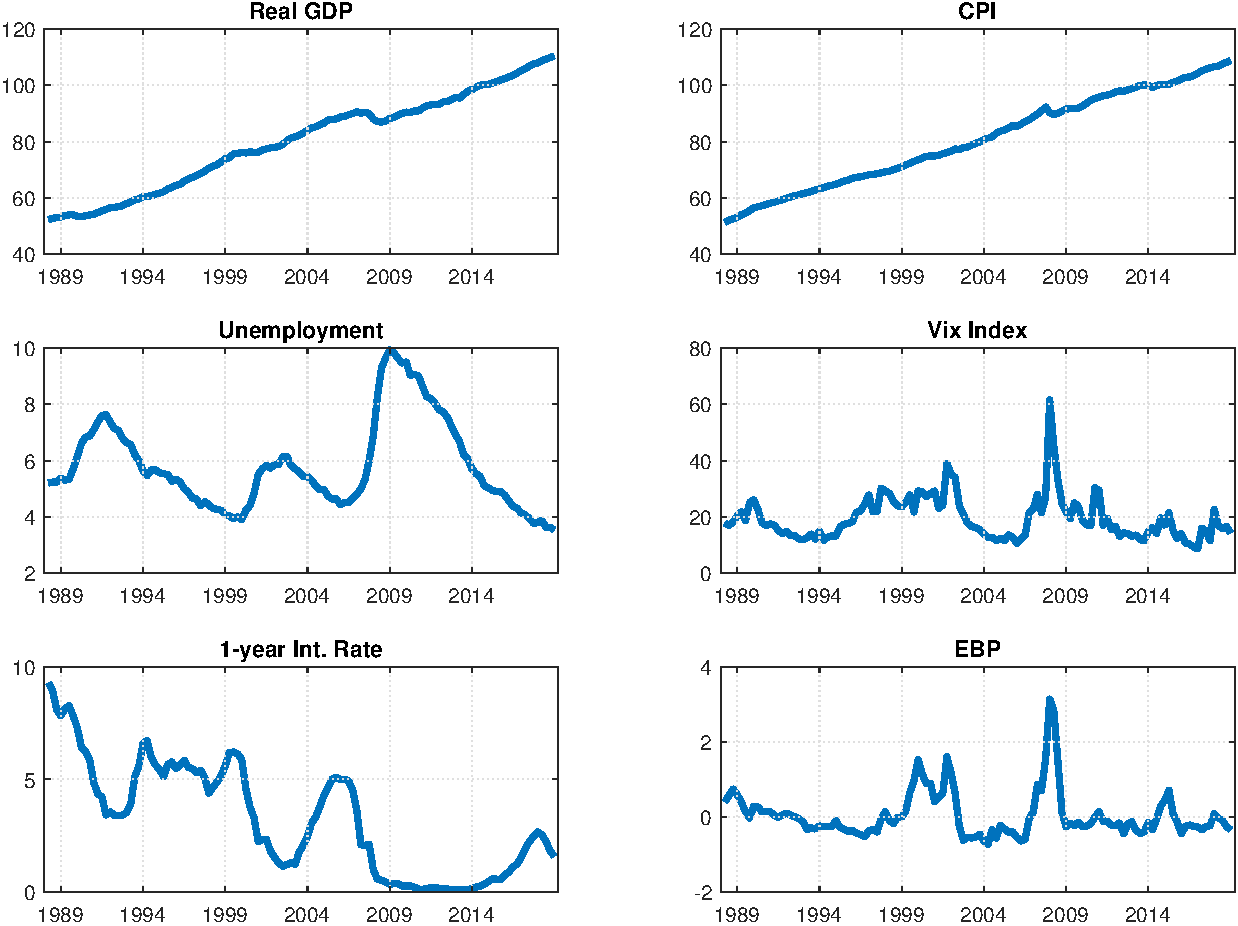
\includegraphics[width=\textwidth]{DATA_GK}
\end{center}%
\footnotesize{{\scshape Note.} Raw data for interest rate on US 1-year Treasury bill, industrial production, CPI level and the Excess Bond Premium (GZ) from 1979;M7 to 2015:M3.}
\label{fig:DATA_GK}
\end{minipage}
\end{figure}

Some useful functions are:

\begin{itemize}
\item \texttt{FigSize.m}: allows the user to choose the proportions of the
figure to plot. This is particularly useful when creating figures with many
panels.

\item \texttt{DatesPlot.m}: Adds dates to the horizontal axis of a chart (at
monthly, quarterly, and annual frequency) using a specified number of ticks.

\item \texttt{SaveFigure.m}: saves the chart in the selected format (pdf,
jpg, eps). The function allows the user to save the figure at high quality
standard using the \texttt{export\_fig.m} function created by Oliver
Woodford. Note that you need Ghostscript to be able to use this function.
\end{itemize}

\section{VAR\ estimation {\color{note} {\protect\small {[Matlab]}}}}

To keep the exposition as simple as possible, we start from a vary stylized
VAR(1) with a constant and only two endogenous variables, namely the monthly
growth rate of industrial production and the monthly growth rate of the CPI\
(i.e. monthly inflation):%
\begin{equation*}
\begin{bmatrix}
IP_{t} \\
R_{t}%
\end{bmatrix}%
=%
\begin{bmatrix}
\alpha ^{IP} \\
\alpha ^{R}%
\end{bmatrix}%
+\left[
\begin{array}{cc}
\phi _{11} & \phi _{12} \\
\phi _{21} & \phi _{22}%
\end{array}%
\right]
\begin{bmatrix}
IP_{t-1} \\
R_{t-1}%
\end{bmatrix}%
+%
\begin{bmatrix}
u_{t}^{IP} \\
u_{t}^{R}%
\end{bmatrix}%
.
\end{equation*}%
While such a simple VAR\ cannot realistically describe the complex
interactions of the US\ economy, it is a useful device to understand the
functioning of the VT\ codes and the workings of VAR\ models more in general.

In the VT, a VAR\ model can be estimated with a simple line of code, using
the \texttt{VARmodel.m} function. To do that you need to specify a matrix
including the endogenous variables (\texttt{ENDO}), whether you want
deterministic variables, like a constant or a trend for example (\texttt{det}%
), and the number of lags of the VAR (\texttt{nlags}). In the example, I\
specify a simple bivariate VAR(12) in industrial production and interest
rates, with a constant.\footnote\textcolor{matlabgreen}{\% VAR ESTIMATION }\\
\hspace{1mm}\textcolor{matlabgreen}{\%--------------------------------------------------------------------------  }\\
\hspace{1mm}\textcolor{matlabgreen}{\% Set the deterministic variable in the VAR (1=constant, 2=trend) }\\
\hspace{1mm}det = 1; \\
\hspace{1mm}\textcolor{matlabgreen}{\% Set number of nlags }\\
\hspace{1mm}nlags = 12; \\
\hspace{1mm}\textcolor{matlabgreen}{\% Estimate VAR by OLS }\\
\hspace{1mm}[VAR, VARopt] = VARmodel(ENDO,nlags,det); \\
\hspace{1mm}disp(VAR) \\
\hspace{1mm}disp(VARopt) \\
\hspace{1mm}\textcolor{matlabgreen}{\% Add variable names to VARopt }\\
\hspace{1mm}VARopt.vnames = VARvnames; \\
\hspace{1mm}VARopt.figname= \textcolor{matlabpurple}{'graphics/'}; \\
\hspace{1mm}\textcolor{matlabgreen}{\% Print at screen and create table }\\
\hspace{1mm}[TABLE, beta] = VARprint(VAR,VARopt,2); \\
}

The cell array \texttt{VARvnames} defines the list of endogenous variables
that will be used to estimate the VAR model (in this case, industrial
production and interest rates, namely a subset of the data in \texttt{DATA}%
). The chosen data is then stored in the matrix \texttt{ENDO}. The
convention in the VT is that each column is a variable and each row is an
observation (with no missing observations allowed). That is:%
\begin{equation*}
\text{\texttt{ENDO}}=\left[
\begin{array}{cc}
IP_{1} & R_{1} \\
IP_{2} & R_{2} \\
... & ... \\
IP_{T} & R_{T}%
\end{array}%
\right] =\left( IP_{t}^{\prime },R_{t}^{\prime }\right) =x_{t}^{\prime }.
\end{equation*}%
This convention implies that, using the notation defined in the previous
section, \texttt{ENDO}$\ =x_{t}^{\prime }$.

The VAR\ can then be estimated in a few lines of code.

\todo[color=script!80,inline]{\ttfamily
\hspace{1mm}\textcolor{matlabgreen}{\%}\textcolor{matlabgreen}{\% VAR ESTIMATION }\\
\hspace{1mm}\textcolor{matlabgreen}{\%--------------------------------------------------------------------------  }\\
\hspace{1mm}\textcolor{matlabgreen}{\% Set the deterministic variable in the VAR (1=constant, 2=trend) }\\
\hspace{1mm}det = 1; \\
\hspace{1mm}\textcolor{matlabgreen}{\% Set number of nlags }\\
\hspace{1mm}nlags = 12; \\
\hspace{1mm}\textcolor{matlabgreen}{\% Estimate VAR by OLS }\\
\hspace{1mm}[VAR, VARopt] = VARmodel(ENDO,nlags,det); \\
\hspace{1mm}disp(VAR) \\
\hspace{1mm}disp(VARopt) \\
\hspace{1mm}\textcolor{matlabgreen}{\% Add variable names to VARopt }\\
\hspace{1mm}VARopt.vnames = VARvnames; \\
\hspace{1mm}VARopt.figname= \textcolor{matlabpurple}{'graphics/'}; \\
\hspace{1mm}\textcolor{matlabgreen}{\% Print at screen and create table }\\
\hspace{1mm}[TABLE, beta] = VARprint(VAR,VARopt,2); \\
}

The results of the VAR estimation are stored in the structures \texttt{VAR}
and \texttt{VARopt}. The structure \texttt{VAR}\ includes all the estimation
results. These can be seen by executing the command \colorbox{script!80}{%
\texttt{disp(VARprint(VAR)}} which prints the following output in the
command window:

\setlength{\parindent}{.2cm}
\begin{verbatim}
>> disp(VAR)
         ENDO: [396x2 double]
         nlag: 12
        const: 1
         EXOG: []
         nobs: 384
         nvar: 4
      nvar_ex: 0
      nlag_ex: 0
       ncoeff: 24
    ntotcoeff: 25
          eq1: [1x1 struct]
          eq2: [1x1 struct]
          eq3: [1x1 struct]
          eq4: [1x1 struct]
           Ft: [49x4 double]
            F: [4x49 double]
        sigma: [4x4 double]
        resid: [384x4 double]
            X: [384x49 double]
            Y: [384x4 double]
        Fcomp: [48x48 double]
       maxEig: 0.9974
           Fp: [4x4x12 double]
            B: []
      BfromSR: []
          PSI: []
\end{verbatim}

\setlength{\parindent}{.0cm}

The structure \texttt{VAR} includes all the inputs to the \texttt{VARmodel.m}
function, such as the matrix of endogenous variables (\texttt{VAR.ENDO}),
the number of lags (\texttt{VAR.nlags}), and the number of endogenous
variables\ (\texttt{VAR.nvar}). But also includes the estimation output. For
example:

\begin{itemize}
\item The matrix \texttt{VAR.F} collects the estimated coefficients
following the notation in (\ref{eq:var_red_b}), namely we have that \texttt{%
VAR.F}$=\Phi $. For a VAR with $1$ lags and $2$ variables plus a constant,
this means that \texttt{VAR.F} is a $2\times (1\times 2+1)$ matrix.

\item The covariance matrix of the VAR residuals defined by (\ref%
{eq:var_red_cov}) is instead stored in \texttt{VAR.sigma}$=\Sigma _{u}$, of
size $2\times 2$.

\item Note that the structural impact matrix \texttt{VAR.B}$\ =B$, which we
defined in equation (\ref{eq:struct_var}), is empty.\ This is because, for
the moment we estimated only the reduced form VAR (1). The next sections
will show how, with additional assumptions, the also the structural form of
the VAR can be recovered.
\end{itemize}

Other outputs are the OLS\ equation-by-equation estimation results
(structures \texttt{VAR.eq}), the VAR\ companion matrix (\texttt{VAR.Fcomp}%
), the maximum eigenvalue of the VAR\ (\texttt{VAR.maxEig}), etc.\

The structure \texttt{VARopt} includes a few auxiliary variables that are
created automatically by the \texttt{VARmodel.m} function and will be needed
below for the calculation of impulse responses, variance decompositions,
etc. The variables stored in \texttt{VARopt} can be seen by executing the
command \colorbox{script!80}{\texttt{disp(VARopt)}}, which prints the
following output in the Matlab command window:
\begin{verbatim}
>> disp(VARopt)
       vnames: []
    vnames_ex: []
       snames: []
       nsteps: 40
       impact: 0
         shut: 0
        ident: 'oir'
       recurs: 'wold'
       ndraws: 100
         pctg: 95
       method: 'bs'
         pick: 0
      quality: 0
     suptitle: 0
    firstdate: []
    frequency: 'q'
      figname: []
\end{verbatim}

These variables include the number of steps for impulse response functions
and variance decompositions (\texttt{nsteps}), the labels of the endogenous
or exogenous variables for plots (\texttt{vnames} and \texttt{vnames\_ex}),
the confidence levels for the computation of error bands (\texttt{pctg}),
etc. While some variables are automatically created by the VARmodel
function, some other variables need to be inputted by the user.\ For example:

\begin{itemize}
\item \colorbox{script!80}{\texttt{VARopt.vnames = VARvnames}} stores in
\texttt{VARopt} the endogenous variables' names.

\item \colorbox{script!80}{\texttt{VARopt.figname =
'graphics/'}} stores in \texttt{VARopt} the name of the folder where all
figures will be saved.
\end{itemize}

So that when executing \colorbox{script!80}{\texttt{disp(VARopt)}} we now
get:
\begin{verbatim}
>> disp(VARopt)
       vnames: {'gs1'  'logcpi'  'logip'  'ebp'}
    vnames_ex: []
       snames: []
       nsteps: 40
       impact: 0
         shut: 0
        ident: 'oir'
       recurs: 'wold'
       ndraws: 100
         pctg: 95
       method: 'bs'
         pick: 0
      quality: 0
     suptitle: 0
    firstdate: []
    frequency: 'q'
      figname: 'graphics/'
\end{verbatim}

\section{The Identification\ Problem {\color{note} {\protect\small {[Notes]}}%
}}

In the previous section we have seen that we can estimate the following
reduced form VAR with OLS:%
\begin{equation}
\begin{bmatrix}
IP_{t} \\
R_{t}%
\end{bmatrix}%
=%
\begin{bmatrix}
\alpha ^{IP} \\
\alpha ^{R}%
\end{bmatrix}%
+\left[
\begin{array}{cc}
\phi _{11} & \phi _{12} \\
\phi _{21} & \phi _{22}%
\end{array}%
\right]
\begin{bmatrix}
IP_{t-1} \\
R_{t-1}%
\end{bmatrix}%
+%
\begin{bmatrix}
u_{t}^{IP} \\
u_{t}^{R}%
\end{bmatrix}%
.  \label{eq:red_2var}
\end{equation}%
Now, imagine that you are asked to estimate the effect of a monetary policy
shock on industrial production. Unfortunately, the reduced form innovation
to the interest rate ($u_{t}^{R}$) is not going to help us. The reason is
that, as we discussed in Section \ref{sec:basics}, $u_{t}^{R}$ is a linear
combination of the true structural shocks in the economy. So, it does not
tell us anything about how monetary policy affects output.

To see that more clearly, assume that the `true' model of the economy is
given by the following structural VAR:%
\begin{equation}
\begin{bmatrix}
IP_{t} \\
R_{t}%
\end{bmatrix}%
=%
\begin{bmatrix}
\alpha ^{IP} \\
\alpha ^{R}%
\end{bmatrix}%
+\left[
\begin{array}{cc}
\phi _{11} & \phi _{12} \\
\phi _{21} & \phi _{22}%
\end{array}%
\right]
\begin{bmatrix}
IP_{t-1} \\
R_{t-1}%
\end{bmatrix}%
+\left[
\begin{array}{cc}
b_{11} & b_{12} \\
b_{21} & b_{22}%
\end{array}%
\right]
\begin{bmatrix}
\varepsilon _{t}^{Demand} \\
\varepsilon _{t}^{Mon.\ Pol}%
\end{bmatrix}%
,  \label{eq:struct_2var}
\end{equation}%
where the matrix $B$ and the structural shocks $\varepsilon $ are
unobserved. The SVAR\ in (XX) assumes that time series of industrial
production and interest rates are driven by a combination of demand and
monetary policy shocks.\footnote{%
Again this is not a very realistic assumption, but it simplifies the math
that follows. A more realistic VAR\ would have included more varibles and
more shocks.} It is obvious that the reduced form innovation to the interest
rate, $u_{t}^{R}$, is a linear combination of all shocks, and not just the
monetary policy shock.

To answer the question of what are the effects of monetary policy on the
economy, we need to find the values of the $B$ matrix. This is known as the
identification problem. For example, the coefficients $b_{12}$ and $b_{22}$
give us the impact effect of monetary policy on industrial production and
interest rates. The matrix of coefficient $\Phi $, which we estimated in the
reduced form VAR, can then be used to trace out the dynamic effects of
monetary policy on the economy beyond the impact effect.

So, how can we go from the reduced form representation to the structural
representation of the VAR? We have seen above that $u_{t}=B\varepsilon _{t}$%
. so that we can write:%
\begin{equation}
\Sigma _{u}=E\left[ u_{t}u_{t}^{\prime }\right] =E\left[ B\varepsilon
_{t}\left( B\varepsilon _{t}\right) ^{\prime }\right] =B\Sigma _{\varepsilon
}B^{\prime }=BB^{\prime }.  \label{eq:red2struct_1}
\end{equation}%
where remember that $\Sigma _{\varepsilon }=I$. This means that there is a
mapping between the estimated covariance matrix of the reduced form
residuals ($\Sigma _{u}$)\ and the unobserved matrix of structural impact
coefficients ($B$). The identification problem simply boils down to finding
a $B$ matrix that satisfies $\Sigma _{u}=BB^{\prime }$.

Unfortunately this is not as easy as it sounds. We can think of (\ref{eq:2})
as a system of nonlinear equations in the $4$ unknown coefficients of the $B$
matrix. The problem the $\Sigma _{u}$ matrix, given its symmetric nature,
leads to only $3$ independent restrictions. In other words, we have
\begin{equation}
\left[
\begin{array}{cc}
\sigma _{y}^{2} & \sigma _{yr}^{2} \\
- & \sigma _{r}^{2}%
\end{array}%
\right] =\left[
\begin{array}{cc}
b_{11} & b_{12} \\
b_{21} & b_{22}%
\end{array}%
\right] \left[
\begin{array}{cc}
b_{11} & b_{21} \\
b_{12} & b_{22}%
\end{array}%
\right] ,  \label{eq:red2struct_2}
\end{equation}%
which can be rewritten as the following system of equations:%
\begin{equation}
\begin{array}{l}
\sigma _{y}^{2}=b_{11}^{2}+b_{12}^{2} \\
\sigma _{yr}^{2}=b_{11}b_{21}+b_{12}b_{22} \\
\sigma _{yr}^{2}=b_{11}b_{21}+b_{12}b_{22} \\
\sigma _{r}^{2}=b_{21}^{2}+b_{22}^{2}%
\end{array}
\label{eq:red2struct_3}
\end{equation}%
Note that, because of the symmetry of the $\Sigma _{u}$ matrix, the second
and the third equation are identical. This means that we are left with $4$
unknowns (the $b$'s) but only $3$ equations. The system is clearly
under-identified, meaning that there are infinite combination of the $b$'s
that solve the system of equations (\ref{eq:red2struct_3}).

How to solve a system of 3 equations in 4 unknowns? The solution typically
is to use economic theory to derive an additional condition that allows us
to recover a fourth equation -- and therefore, solve the system of equations
(\ref{eq:red2struct_3}).\ For example, if you believe that monetary policy
works with a lag and has no effect on ouput on impact, you can impose $%
b_{21}=0$. If added to the system (\ref{eq:red2struct_3}), this equation
allows for a unique solution of the elements of $B$.

There are many ways of solving the identification problem described above.
In the following section, we will cover a few popular identification
schemes, and how thy can be implemented in the VT.

\section{Common Identification schemes}

Many solutions have been developed in the literature to address the
identification problem described in the previous section. In this section,
we go through the some popular ones namely, zero (recursive)\
contemporaneous restrictions, zero (recursive)\ long-run restrictions, sign
restrictions, external instruments, combining sign restrictions and external
instruments.

\subsection{Identification by zero contemporaneous restrictions}

Identification using zero contemporaneous restrictions (also known as
Cholesky identification, for a reason that will be clear in a second) were
developed by Sims1980, and are by far the most commonly used identification
scheme used in the literature. In a recursive SVAR, identification is
achieved by assuming that some shocks have zero contemporaneous effect on
some of the endogenous variables. This amounts to setting some of the
non-diagonal elements of the $B$ matrix to zero -- therefore reducing the
number of unknown coefficients.

Typically, it is assumed that the first variable in the system is only
affected by the first structural shock, the second is contemporaneously
affected by the first and second structural shock, and so on. In our
example, that means to assume that the structural VAR\ is
\begin{equation}
\begin{bmatrix}
IP_{t} \\
R_{t}%
\end{bmatrix}%
=%
\begin{bmatrix}
\alpha ^{IP} \\
\alpha ^{R}%
\end{bmatrix}%
+\left[
\begin{array}{cc}
\phi _{11} & \phi _{12} \\
\phi _{21} & \phi _{22}%
\end{array}%
\right]
\begin{bmatrix}
IP_{t-1} \\
R_{t-1}%
\end{bmatrix}%
+\left[
\begin{array}{cc}
b_{11} & 0 \\
b_{21} & b_{22}%
\end{array}%
\right]
\begin{bmatrix}
\varepsilon _{t}^{Demand} \\
\varepsilon _{t}^{Mon.\ Pol}%
\end{bmatrix}%
,
\end{equation}%
where note that the industrial production is not contemporaneously affected
by the monetary policy shock (while interest rates are contemporaneously
affected by both the demand and the monetary policy shock). This assumption
could be justified by the fact that monetary policy takes time to affect
real variables like industrial production.

What are the implications for the identification problem described above?
The simple answer is that we now have 3 instead of 4 structural parameters
to estimate, and 3 restrictions implied by the reduced form covariance
matrix. That is, the system of equations (\ref{eq:red2struct_3}) now becomes:%
\begin{equation}
\left\{
\begin{array}{l}
\sigma _{y}^{2}=b_{11}^{2}, \\
\sigma _{yr}^{2}=b_{11}b_{21}, \\
\sigma _{r}^{2}=b_{21}^{2}+b_{22}^{2}.%
\end{array}%
\right.   \label{eq:red2struct_4}
\end{equation}%
which can be easily solved to get:%
\begin{equation*}
\left\{
\begin{array}{c}
b_{11}=\sigma _{y}^{2}, \\
b_{21}=\sigma _{yr}^{2}/\sigma _{y}^{2}, \\
b_{22}=\sqrt{\sigma _{r}^{2}-\frac{\sigma _{yr}^{2}}{\sigma _{y}^{2}}.}%
\end{array}%
\right.
\end{equation*}%
The VAR\ is identified! This means that it is possible to compute the \emph{%
impact} impulse response of all endogenous variables by simply looking at
the estimated $B$\ matrix. For example, consider a one standard deviation
shock to monetary policy, i.e. $\varepsilon _{t}^{Mon.\ Pol}=1$. Using the
structural VAR\ representation
\begin{equation*}
\begin{bmatrix}
IP_{t} \\
R_{t}%
\end{bmatrix}%
=%
\begin{bmatrix}
\alpha ^{IP} \\
\alpha ^{R}%
\end{bmatrix}%
+\left[
\begin{array}{cc}
\phi _{11} & \phi _{12} \\
\phi _{21} & \phi _{22}%
\end{array}%
\right]
\begin{bmatrix}
IP_{t-1} \\
R_{t-1}%
\end{bmatrix}%
+\left[
\begin{array}{cc}
\sigma _{y}^{2} & 0 \\
\sigma _{yr}^{2}/\sigma _{y}^{2} & \sqrt{\sigma _{r}^{2}-\frac{\sigma
_{yr}^{2}}{\sigma _{y}^{2}}}%
\end{array}%
\right]
\begin{bmatrix}
\varepsilon _{t}^{Demand} \\
\varepsilon _{t}^{Mon.\ Pol}%
\end{bmatrix}%
.
\end{equation*}%
we get:%
\begin{eqnarray*}
IP_{t} &=&0, \\
R_{t} &=&\sqrt{\sigma _{r}^{2}-\frac{\sigma _{yr}^{2}}{\sigma _{y}^{2}}}.
\end{eqnarray*}%
A one standard deviation shock to aggregate demand ($\varepsilon
_{t}^{Demand}=1$) in $t$ leads to%
\begin{eqnarray*}
IP_{t} &=&\sigma _{y}^{2}, \\
R_{t} &=&\sigma _{yr}^{2}/\sigma _{y}^{2}.
\end{eqnarray*}

\subsection{Identification by zero long-run restrictions}

Identification using zero contemporaneous restrictions (also known as
recursive identification, for a reason that will be

\subsection{Variance decompositions}

\subsection{Historical decompositions}

\bibliographystyle{chicago}
\bibliography{BIBLIO}

\appendix

\section{Appendix}

\subsection{The Identification\ Problem {\color{note}
{\protect\small
{[Notes]}}}}

In the previous section we have seen how to estimate a reduced form VAR.
Ignoring lagged variables beyond order 1 for ease of notation, we estimated
the following:%
\begin{equation}
\begin{bmatrix}
R_{t} \\
IP_{t} \\
CPI_{t} \\
EBP_{t}%
\end{bmatrix}%
=\left[
\begin{array}{cccc}
\phi _{11} & \phi _{12} & \phi _{13} & \phi _{14} \\
\phi _{21} & \phi _{22} & \phi _{23} & \phi _{24} \\
\phi _{31} & \phi _{12} & \phi _{33} & \phi _{34} \\
\phi _{41} & \phi _{22} & \phi _{43} & \phi _{44}%
\end{array}%
\right]
\begin{bmatrix}
R_{t-1} \\
IP_{t-1} \\
CPI_{t-1} \\
EBP_{t-1}%
\end{bmatrix}%
+\text{other lags}+%
\begin{bmatrix}
u_{t}^{R} \\
u_{t}^{IP} \\
u_{t}^{CPI} \\
u_{t}^{EBP}%
\end{bmatrix}%
,
\end{equation}%
Now, imagine that you are asked to estimate the effect of a monetary policy
shock to industrial production and consumer prices. Unfortunately, the
reduced form innovation to the interest rate ($u_{t}^{R}$) is not going to
help us. The reason is that, as we discussed in Section \ref{sec:basics}, $%
u_{t}^{R}$ is a linear combination of the true structural shocks in the
economy. So, it does not tell us anything about how monetary policy affects
output and prices.

To see that more clearly, assume that the `true' model of the economy is
given by the following structural VAR:%
\begin{equation}
\begin{bmatrix}
R_{t} \\
IP_{t} \\
CPI_{t} \\
EBP_{t}%
\end{bmatrix}%
=\text{all lags}+\left[
\begin{array}{cccc}
b_{11} & b_{12} & b_{13} & b_{14} \\
b_{21} & b_{22} & b_{23} & b_{24} \\
b_{31} & b_{12} & b_{33} & b_{34} \\
b_{41} & b_{22} & b_{43} & b_{44}%
\end{array}%
\right]
\begin{bmatrix}
\varepsilon _{t}^{Mon.\ Pol} \\
\varepsilon _{t}^{Demand} \\
\varepsilon _{t}^{Supply} \\
\varepsilon _{t}^{Financial}%
\end{bmatrix}%
,  \label{eq:GK_VAR}
\end{equation}%
where the matrix $B$ and the structural shocks $\varepsilon $ are
unobserved. The SVAR\ in (XX) assumes that time series of interest rates,
industrial production, consumer prices and the excess bond premium are
driven by a combination of monetary, demand, supply and financial shocks. It
is obvious that the reduced form innovation to the interest rate, $u_{t}^{R}$%
, is a linear combination of all shocks, and not just the monetary policy
shock.

To answer the question of what are the effects of monetary policy on the
economy, we need to find the values of the $B$ matrix. This is known as the
identification problem. For example, the coefficients $b_{11}$, $b_{21}$, $%
b_{31}$, and $b_{41}$ give us the impact effect of monetary policy on all
variables. The matrix of coefficient $\Phi $, which we estimated in the
reduced form VAR, can then be used to trace out the dynamic effects of
monetary policy on the economy beyond the impact effect.

So, how can we go from the reduced form representation to the structural
representation of the VAR? From equation (\ref{eq:var_reduced_c}) we know
that:%
\begin{equation}
\hat{\Sigma}_{u}=E\left[ \hat{u}_{t}\hat{u}_{t}^{\prime }\right] =E\left[
B\varepsilon \left( B\varepsilon \right) ^{\prime }\right] =B\Sigma
_{\varepsilon }B^{\prime }=BB^{\prime }.  \label{eq:2}
\end{equation}%
where remember that $\Sigma _{\varepsilon }=I$. This means that there is a
mapping between the estimated covariance matrix of the reduced form
residuals ($\hat{\Sigma}_{u}$)\ and the unobserved matrix of structural
impact coefficients. We can think of (\ref{eq:2}) as a system of nonlinear
equations in the $4\times 4$ unknown coefficients of the $B$ matrix. The
problem the $\Sigma _{u}$ matrix ---given its symmetric nature--- would
contain only $4+(4\times 3)/2$ parameters. In other words, we have
\begin{equation*}
\mathbf{\Sigma }_{u}=\left[
\begin{array}{cccc}
\sigma _{y}^{2} & \sigma _{yr}^{2} & \sigma _{13}^{2} & \sigma _{14}^{2} \\
- & \sigma _{r}^{2} & \sigma _{23}^{2} & \sigma _{24}^{2} \\
- & - & \sigma _{3}^{2} & \sigma _{34}^{2} \\
- & - & - & \sigma _{4}^{2}%
\end{array}%
\right] =\left[
\begin{array}{cccc}
b_{11} & b_{12} & b_{13} & b_{14} \\
b_{21} & b_{22} & b_{23} & b_{24} \\
b_{31} & b_{12} & b_{33} & b_{34} \\
b_{41} & b_{22} & b_{43} & b_{44}%
\end{array}%
\right] \left[
\begin{array}{cccc}
b_{11} & b_{12} & b_{13} & b_{14} \\
b_{21} & b_{22} & b_{23} & b_{24} \\
b_{31} & b_{12} & b_{33} & b_{34} \\
b_{41} & b_{22} & b_{43} & b_{44}%
\end{array}%
\right] ^{\prime }
\end{equation*}%
which shows that there are 16 unknowns but only 10 independent equations.
The system is clearly under-identified, meaning that we need additional
conditions if we want to recover the structural parameters.

There are many ways of identifying solving the identification problem
described above. In the following section, I will describe a few of the most
popular ones, and how thy can be implemented in the VAR\ Tolbox.

\subsection{Impulse responses}

ZERO LONG-RUN RESTRICTIONS. Similarly to the short-run restrictions,
identification is achieved by making the assumption that some variables of
the VAR\ cannot affect some other variables in the long-run. Specifically we
will assume that the first variable is not affected in the long run by the
others; the second is affected in the long run by the first variable but not
by the others, and so on and so forth.

SIGN RESTRICTIONS. Identification is achieved by restricting the sign of the
responses of selected model variables to structural shocks, using economic
theory as a guidance

\end{document}
